\chapter{Generative models}


\begin{description}
    \item[Generative task] \marginnote{Generative task}
        Given the training data $\{ x^{(i)} \}$, learn its distribution so that a model can sample new examples:
        \[ \hat{x}^{(i)} \sim p_\text{gen}(x; \matr{\theta}) \]

        \begin{figure}[H]
            \centering
            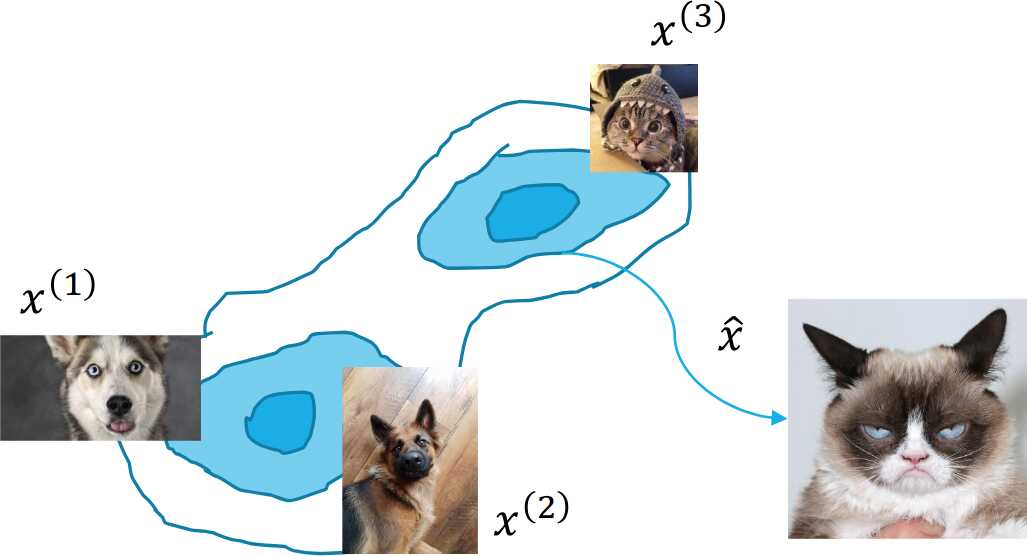
\includegraphics[width=0.4\linewidth]{./img/generative_task.jpg}
        \end{figure}

        \begin{remark}
            Generative tasks are hard as natural images lay on a low dimensional subspace (i.e., only a tiny subset of all the possible RGB images makes sense).

            \begin{figure}[H]
                \centering
                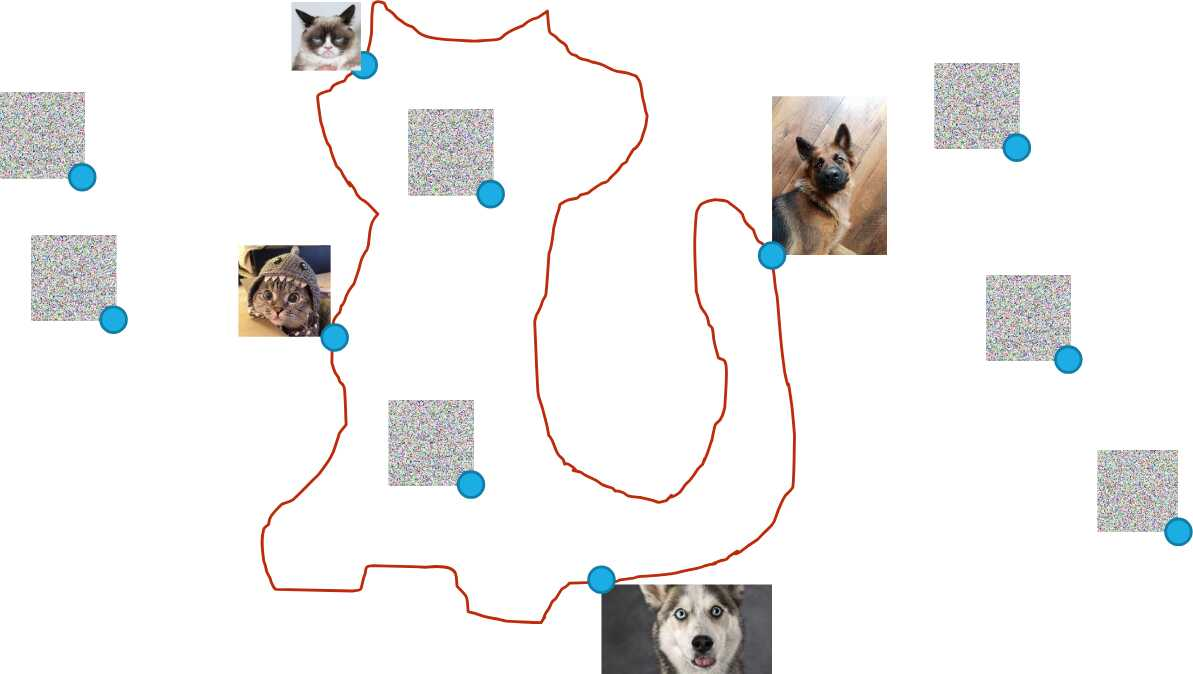
\includegraphics[width=0.6\linewidth]{./img/image_manifold.jpg}
            \end{figure}
        \end{remark}

    \item[Latent vector] \marginnote{Latent vector}
        Low-dimensional representation to encode an image.

        \begin{example}
            Face expression depends on 42 muscles. A latent representation for different poses of a face can be represented with a 42-dimensional vector.
        \end{example}

        It is assumed that the factors of a latent vector are independent or mildly correlated, and can be sampled from a known distribution.

    \item[Generative model] \marginnote{Generative model}
        Model that takes as input a latent representation and maps it into an output image.
        \begin{figure}[H]
            \centering
            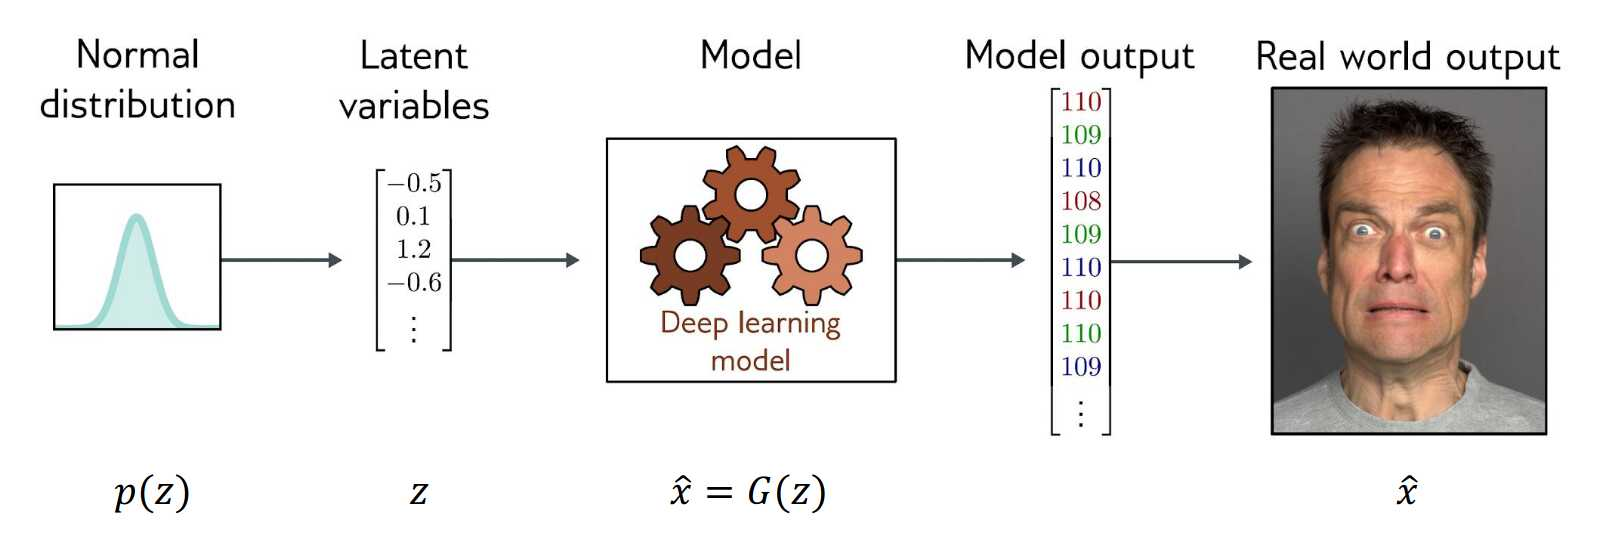
\includegraphics[width=0.7\linewidth]{./img/latent_for_generation.jpg}
        \end{figure}

        \begin{remark}
            An ideal generative model should have the following properties:
            \begin{itemize}
                \item Be computationally efficient when sampling.
                \item Produce high-quality samples.
                \item Represent the entire training distribution.
                \item Produce a plausible output from any latent input. Smooth changes to the input should be reflected on the output.
                \item Have a disentangled latent space (i.e., changing a dimension of the latent space corresponds to interpretable changes in the output image).
                \item Have the possibility to calculate the probability of the produced images (when the model is probabilistic). 
            \end{itemize}
        \end{remark}
\end{description}



\section{Metrics}

\begin{description}
    \item[Expectation/Expected value] \marginnote{Expectation/Expected value}
        Informally, it is the generalization of the weighted average:
        \[ 
            \mathbb{E}_{x \sim p}[ f(\cdot) ] = \sum_{x \in \mathbb{X}} p(x) f(x) 
            \qquad
            \mathbb{E}_{x \sim p}[ f(\cdot) ] = \int_{x \in \mathbb{X}} p(x) f(x) \,dx
        \]

        \begin{description}
            \item[Monte Carlo approximation] \marginnote{Monte Carlo approximation}
                Approximation for expectation using $N$ i.i.d. samples drawn from $p(x)$:
                \[ \mathbb{E}_{x \sim p}[f(\cdot)] \approx \frac{1}{N} \sum_{x_i \sim p(x)} f(x_i) \]
        \end{description}

    \item[Self-information] \marginnote{Self-information}
        Given a probability mass function of an event, the self-information of an event $x$ is defined as:
        \[ I(x) = -\log_b(p(x)) = \log_b\left( \frac{1}{p(x)} \right) \]
        Intuitively, it can be seen as a measure of surprise.

        \begin{remark}
            If $b = 2$, self-information is measured in bits. If $b = e$, it is measured in natural unit of information ($nat$).
        \end{remark}

        \begin{example}
            Consider the toss of a fair coin. The self-information for the outcomes are:
            \[ I(\texttt{heads}) = I(\texttt{tails}) = \log_2\left( \frac{1}{0.5} \right) = 1 \text{ bit} \]
            If the coin is loaded toward tails with probability:
            \[ 
                \prob{\texttt{heads}} = 0.05 
                \qquad 
                \prob{\texttt{heads}} = 0.95 
            \]
            The self-information is:
            \[ 
                I(\texttt{heads}) = \log_2\left( \frac{1}{0.05} \right) = 4.31 \text{ bits}
                \qquad
                I(\texttt{tails}) = \log_2\left( \frac{1}{0.95} \right) = 0.07 \text{ bits}
            \]
        \end{example}

    \item[Entropy] \marginnote{Entropy}
        Expected value of the self-information of a probability mass function:
        \[ H(p(\cdot)) = \mathbb{E}_{x \sim p} \left[ - \log(p(x)) \right] \approx -\sum_{x \in \mathbb{X}} p(x) \log(p(x)) \]
        Intuitively, it measures the average surprise of a distribution.
        
        \begin{example}
            Consider the distribution of a fair, loaded, and constant coin. We have that:
            \begin{descriptionlist}
                \item[Maximum entropy] $H(p_\text{fair}(\cdot)) = 0.5 \log(2) + 0.5 \log(2) = \log(2)$
                \item[Low entropy] $H(p_\text{loaded}(\cdot)) = 0.05 \cdot 4.32 + 0.95 \cdot 0.07 = 0.28$
                \item[Minimum entropy] $H(p_\text{constant}(\cdot)) = 0 + 1 \cdot 0 = 0$
            \end{descriptionlist}
        \end{example}

    \item[Kullback-Leibler (KL) divergence] \marginnote{Kullback-Leibler (KL) divergence}
        Distance between probability distributions:
        \[ 
            \begin{split}
                D_\text{KL}(p || q) &= \mathbb{E}_{x \sim p(x)}\left[ \log(p(x)) - \log(q(x)) \right] = \mathbb{E}_{x \sim p(x)} \left[ \log\left( \frac{p(x)}{q(x)} \right) \right] \\ 
                &\approx \sum_{x \in \mathbb{X}} \left( p(x) \log\left( \frac{p(x)}{q(x)} \right) \right) 
            \end{split}
        \]

        \begin{remark}
            KL divergence only samples from one of the distributions. Therefore, it is not symmetric (i.e., it is not a metric).
        \end{remark}

        \begin{remark}
            KL divergence goes to infinity if $q(x) = 0$ and $p(x) \neq 0$.
        \end{remark}

        \begin{example}
            Consider the following cases of a coin toss:
            \begin{table}[H]
                \centering
                \begin{tabular}{c|c|c}
                    \toprule
                    & Other distribution is loaded & Other distribution is constant \\
                    \midrule
                    $p$ is fair & 
                        $0.5\log\left(\frac{0.5}{0.05}\right) + 0.5\log\left(\frac{0.5}{0.95}\right) = 0.83$ & 
                        $0.5\log\left(\frac{0.5}{0}\right) + 0.5\log\left(\frac{0.5}{1}\right) = +\infty$ \\
                    $q$ is fair & 
                        $0.05\log\left(\frac{0.05}{0.5}\right) + 0.95\log\left(\frac{0.95}{0.5}\right) = 0.49$ &
                        $0\log\left(\frac{0}{0.5}\right) + 1\log\left(\frac{1}{0.5}\right) = 0.69$ \\
                    \bottomrule
                \end{tabular}
            \end{table}
        \end{example}

    \item[Jensen-Shannon (JS) divergence] \marginnote{Jensen-Shannon (JS) divergence}
        Variation of KL divergence to make it symmetric and bounded:
        \[ [0, \log_b(2)] \ni D_\text{JS}(p || q) = \frac{1}{2} D_\text{KL}\left( p || \frac{p+q}{2} \right) + \frac{1}{2} D_\text{KL}\left( q || \frac{p+q}{2} \right) \]

        \begin{remark}
            JS divergence has the highest value when $p$ and $q$ are disjoint (i.e., $p(x) > 0 \Rightarrow q(x) = 0$ or vice versa).
        \end{remark}

        \begin{remark}
            JS divergence is symmetric and respects the triangle inequality.
        \end{remark}
\end{description}


\subsection{Inception score}

\begin{description}
    \item[Inception score (IS)] \marginnote{Inception score (IS)}
        Given a generator and a pre-trained image classifier, Inception score assesses that:
        \begin{itemize}
            \item The generated images are classified by the classifier with a high confidence (i.e., $p_\text{cls}(y | x)$ should have low entropy).
            \item The generated images cover all the classes handled by the classifier (i.e., $p_\text{cls}(y)$ should have high entropy).
        \end{itemize}
        
        Inception score is computed as:
        \[ 
            \begin{split}
                [1, C] \ni IS &= \exp\left( \mathbb{E}_{x_i \sim p_\text{gen}(x)}\Big[ D_\text{KL}\big( p_\text{cls}(y | x_i) \,||\, p_\text{cls}(y) \big) \Big] \right) \\
                &= \exp\left( H(p_\text{cls}(y)) - \mathbb{E}_{x_i \sim p_\text{gen}(x)} \Big[ H(p_\text{cls}(y | x_i)) \Big] \right)
            \end{split}
        \]
        where $p_\text{cls}(y)$ is computed through Monte Carlo approximation:
        \[ 
            p_\text{cls}(y) = \mathbb{E}_{x \sim p_\text{gen}}\left[ p_\text{cls}(y | x) \right]
            \approx \frac{1}{N} \sum_{x_i \sim p_\text{gen}(x)} p_\text{cls}(y | x_i)
        \]

        \begin{remark}
            Inception score has the following problems:
            \begin{itemize}
                \item It uses the Monte Carlo approximation and requires a large sample size.
                \item It is sensitive to the performance of the classifier.
                \item It does not measure generation diversity within a class.
            \end{itemize}
        \end{remark}

        \begin{figure}[H]
            \centering
            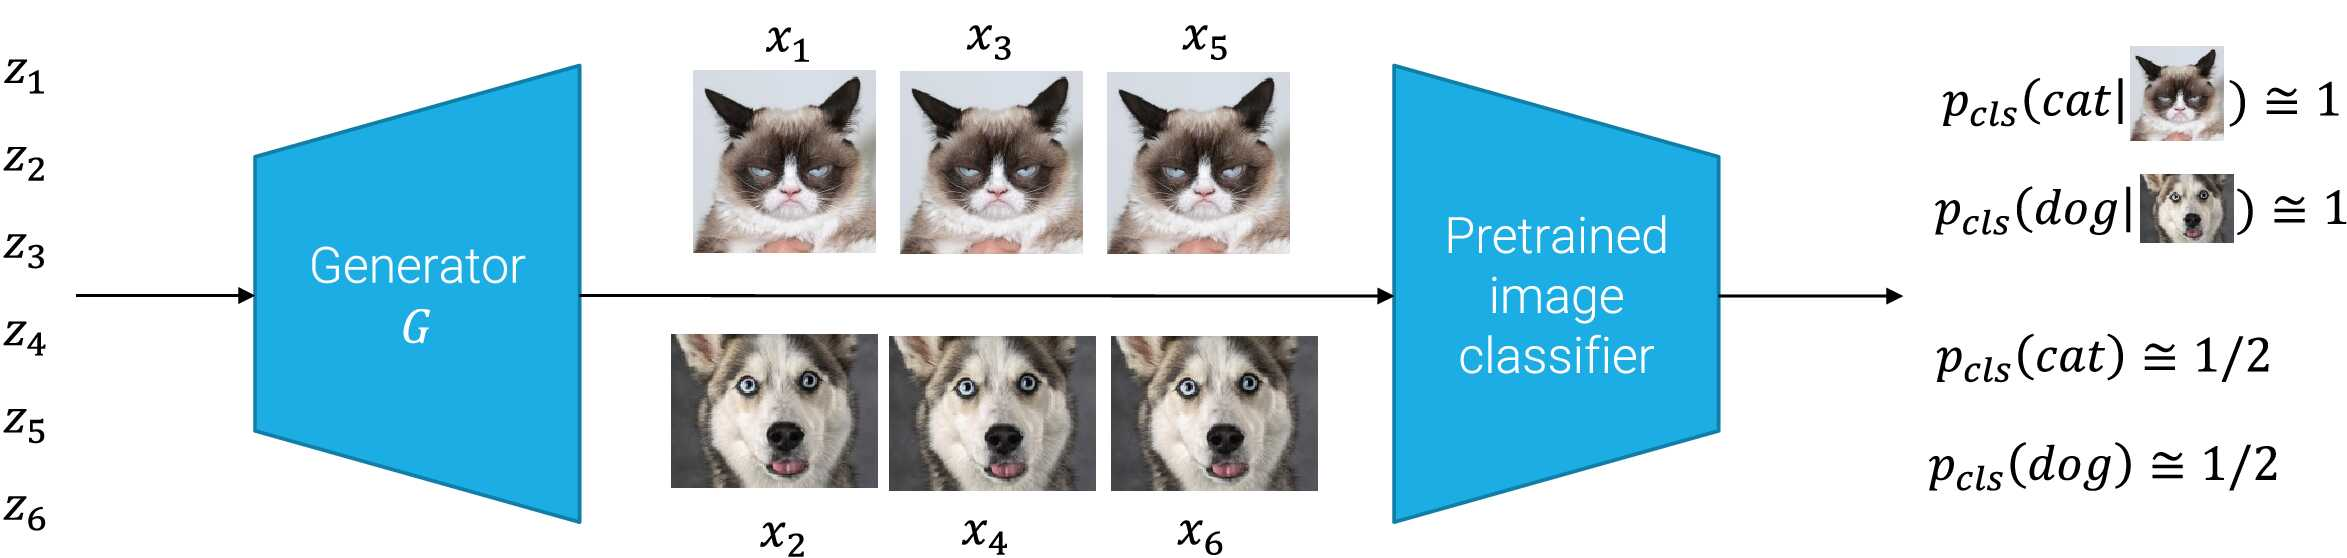
\includegraphics[width=0.8\linewidth]{./img/_inception_score.jpg}
        \end{figure}
\end{description}


\subsection{Fréchet Inception distance}

\begin{description}
    \item[Earth mover's distance (EMD)] \marginnote{Earth mover's distance (EMD)}
        Given two discrete distributions $p$ and $q$, EMD measures the ``work'' needed to match $p$ and $q$ by considering the amount of mass to move and the distance between bins.

        \begin{figure}[H]
            \centering
            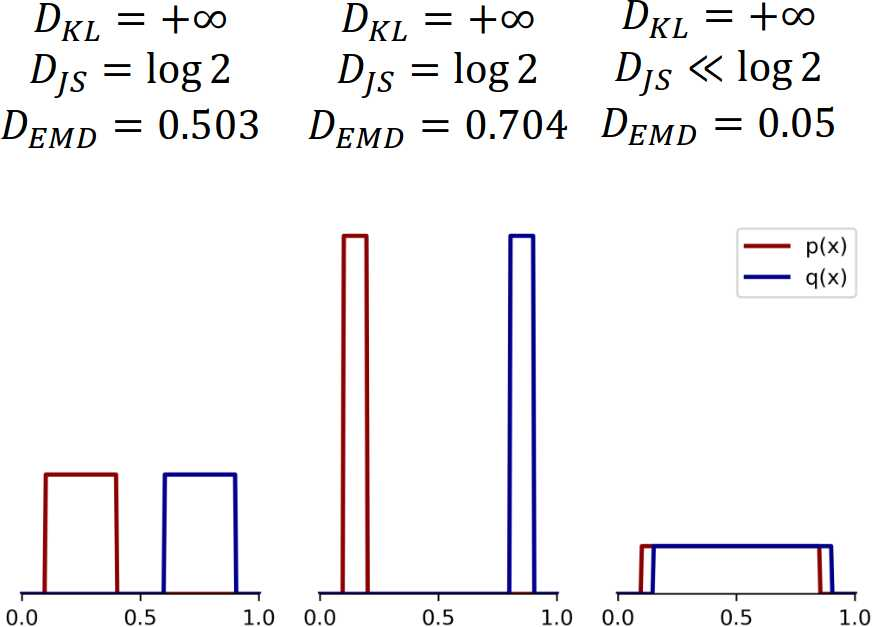
\includegraphics[width=0.4\linewidth]{./img/earth_mover.jpg}
            \caption{
                \parbox[t]{0.8\linewidth}{
                    Three cases of density functions distance. The distributions in the first case are closer than the second one. In the third case, they are mostly overlapping.
                }
            }
        \end{figure}

        Earth mover's distance is formulated as a linear programming problem:
        \[ 
            \begin{split}
                D_\text{EMD}(p || q) = \min_{\matr{P}}\left[ \sum_{i, j} \matr{P}_{i, j} |i-j| \right] \\
                \begin{split}
                    \text{subject to}
                        & \sum_{j} \matr{P}_{i, j} = p(i) \,\land \\
                        & \sum_{i} \matr{P}_{i,j} = q(j) \,\land \\
                        & \matr{P}_{i,j} \geq 0
                \end{split}
            \end{split}
        \]
        where $\matr{P}$ is the transport plan such that $\matr{P}_{i,j}$ indicates the amount of mass to move from bin $i$ (of $p$) to bin $j$ (of $q$).

        \begin{figure}[H]
            \centering
            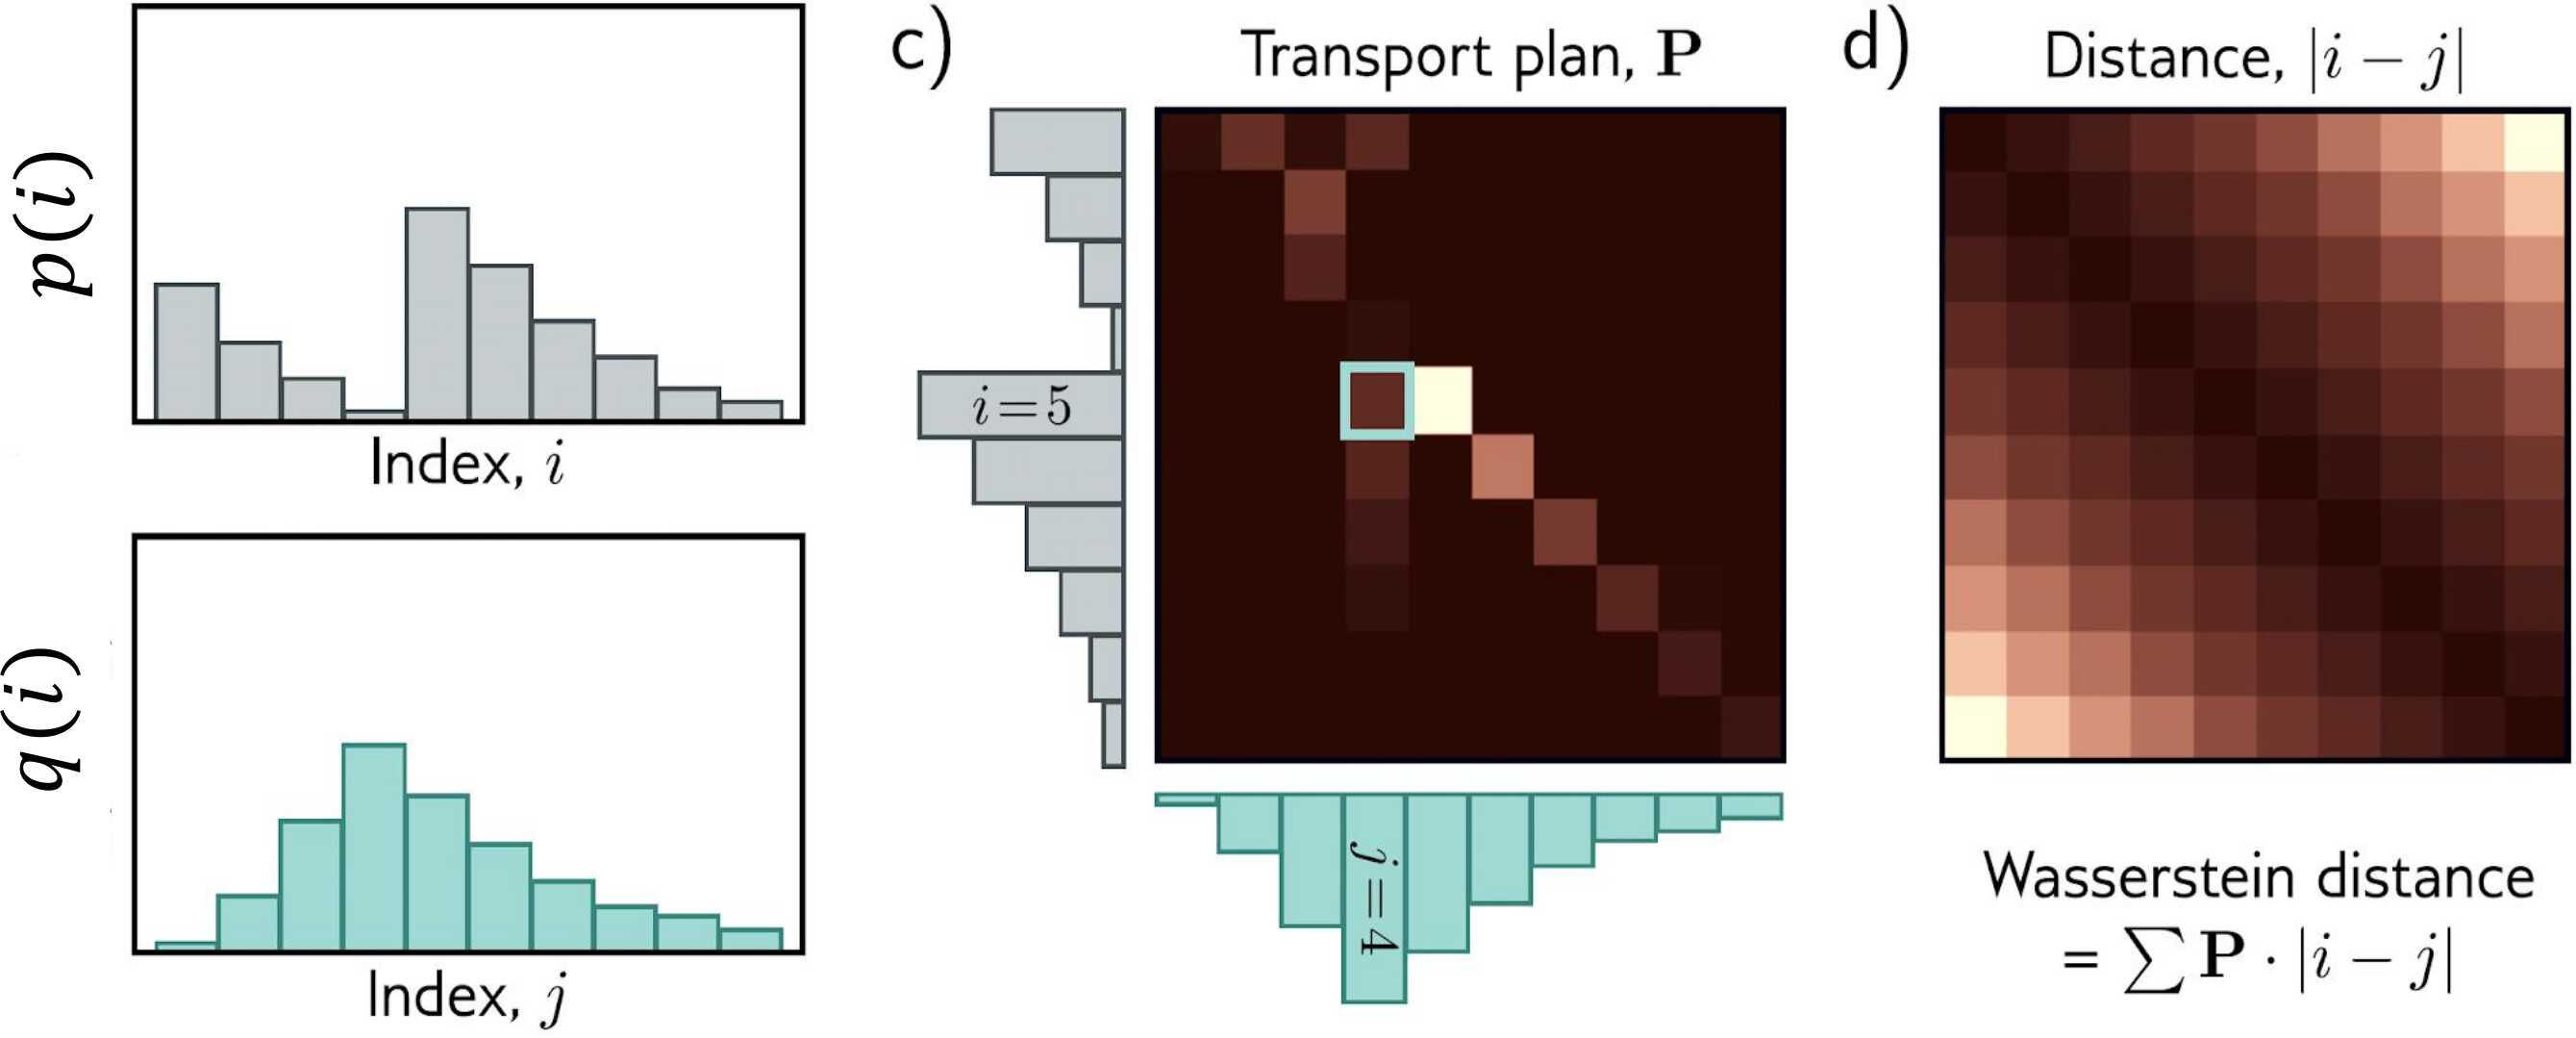
\includegraphics[width=0.6\linewidth]{./img/earth_mover_plan.jpg}
        \end{figure}


    \item[Fréchet Inception distance (FID)] \marginnote{Fréchet Inception distance (FID)}
        \begin{remark}
            In the continuous case, EMD is computed using the Fréchet distance. Applying it as-is has two problems:
            \begin{itemize}
                \item Comparing pixels is not effective.
                \item The distribution of the generated images cannot be analytically determined.
            \end{itemize} 
        \end{remark}

        Fréchet Inception distance is based on two ideas:
        \begin{itemize}
            \item Use the embedding (Inception-v3) of an image instead of pixels.
            \item Assume that the embedding space is a multi-variate Gaussian.
        \end{itemize}
        Given the Gaussians fitted on the embeddings of the real images $\mathcal{N}(x; \mu_r, \Sigma_r)$ and the embeddings of the generated images $\mathcal{N}(x; \mu_g, \Sigma_g)$, FID is computed as:
        \[ 
            D_\text{FR}^2\left[ \mathcal{N}(x; \mu_r, \Sigma_r) || \mathcal{N}(x; \mu_g, \Sigma_g) \right] = \Vert \mu_g - \mu_r \Vert^2_2 + \text{tr}\left( \Sigma_r + \Sigma_g - 2\sqrt{\Sigma_r \Sigma_g} \right)
        \]
    
    \begin{remark}
        FID accounts for both realism and diversity (FID grows if one of the two distribution is more diverse than the other) both across and within classes. However:
        \begin{itemize}
            \item It is sensitive to the pre-trained feature extractor (but it is more robust than Inception score).
            \item It is not possible to distinguish in the final score whether realism or diversity is the problem.
        \end{itemize}
    \end{remark}
\end{description}


\subsection{Manifold precision/recall}

\begin{description}
    \item[Manifold precision] \marginnote{Manifold precision}
        Fraction of generated images that fall into the real data manifold (i.e., realism).

    \item[Manifold recall] \marginnote{Manifold recall}
        Fraction of real images that fall into the generator manifold (i.e., diversity).
\end{description}

\begin{remark}
    These metrics are computed in the embedding space of the images. The manifold is approximated with a hypersphere centered on each embedding with a radius proportional to the distance to the $k$-th nearest neighbor.
\end{remark}

\begin{figure}[H]
    \centering
    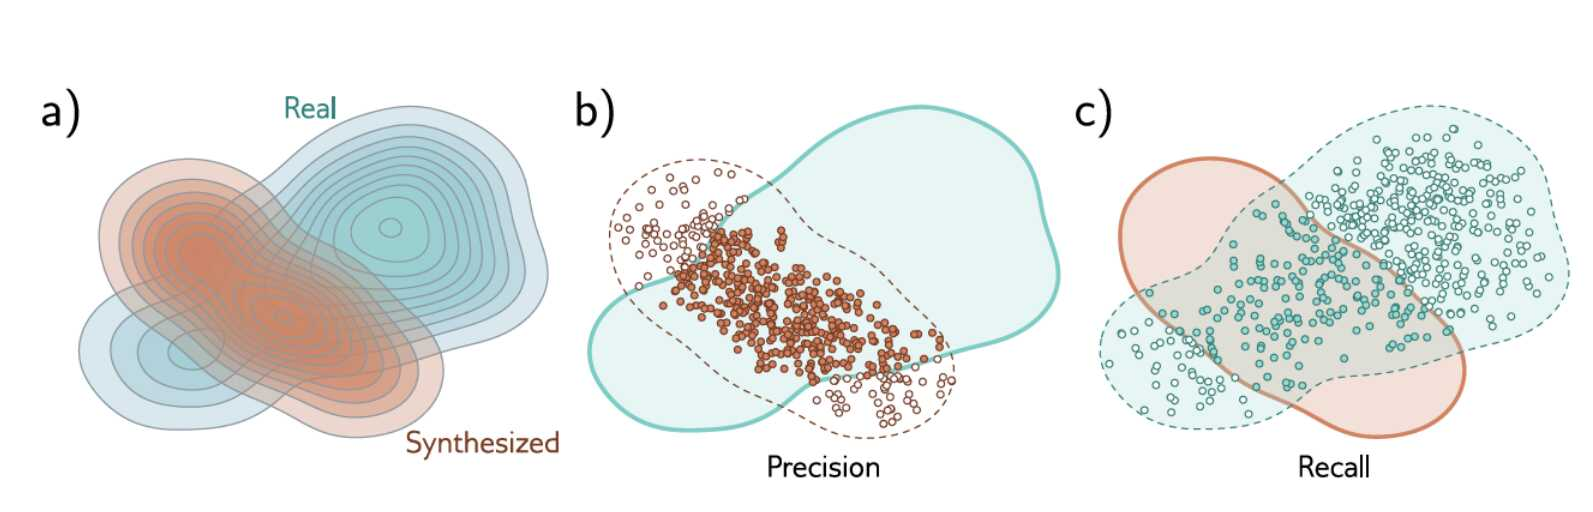
\includegraphics[width=0.8\linewidth]{./img/manifold_precision_recall.jpg}
\end{figure}



\section{Generative adversarial networks}


\begin{description}
    \item[Generative adversarial network (GAN)] \marginnote{Generative adversarial network (GAN)}
        Given:
        \begin{itemize}
            \item A generator $G(z; \theta)$ that takes as input a latent vector $z_i \sim p_\text{lat}(z)$ and produces an image $\hat{x}_j \sim p_\text{gen}(x)$,
            \item A discriminator $D(x; \phi)$ that determines whether $x_i$ is a real image from $p_\text{real}(x)$.
        \end{itemize}
        A generative adversarial network trains both $D$ and $G$ with the aim of making $p_\text{gen}$ converge to $p_\text{real}$.

        \begin{figure}[H]
            \centering
            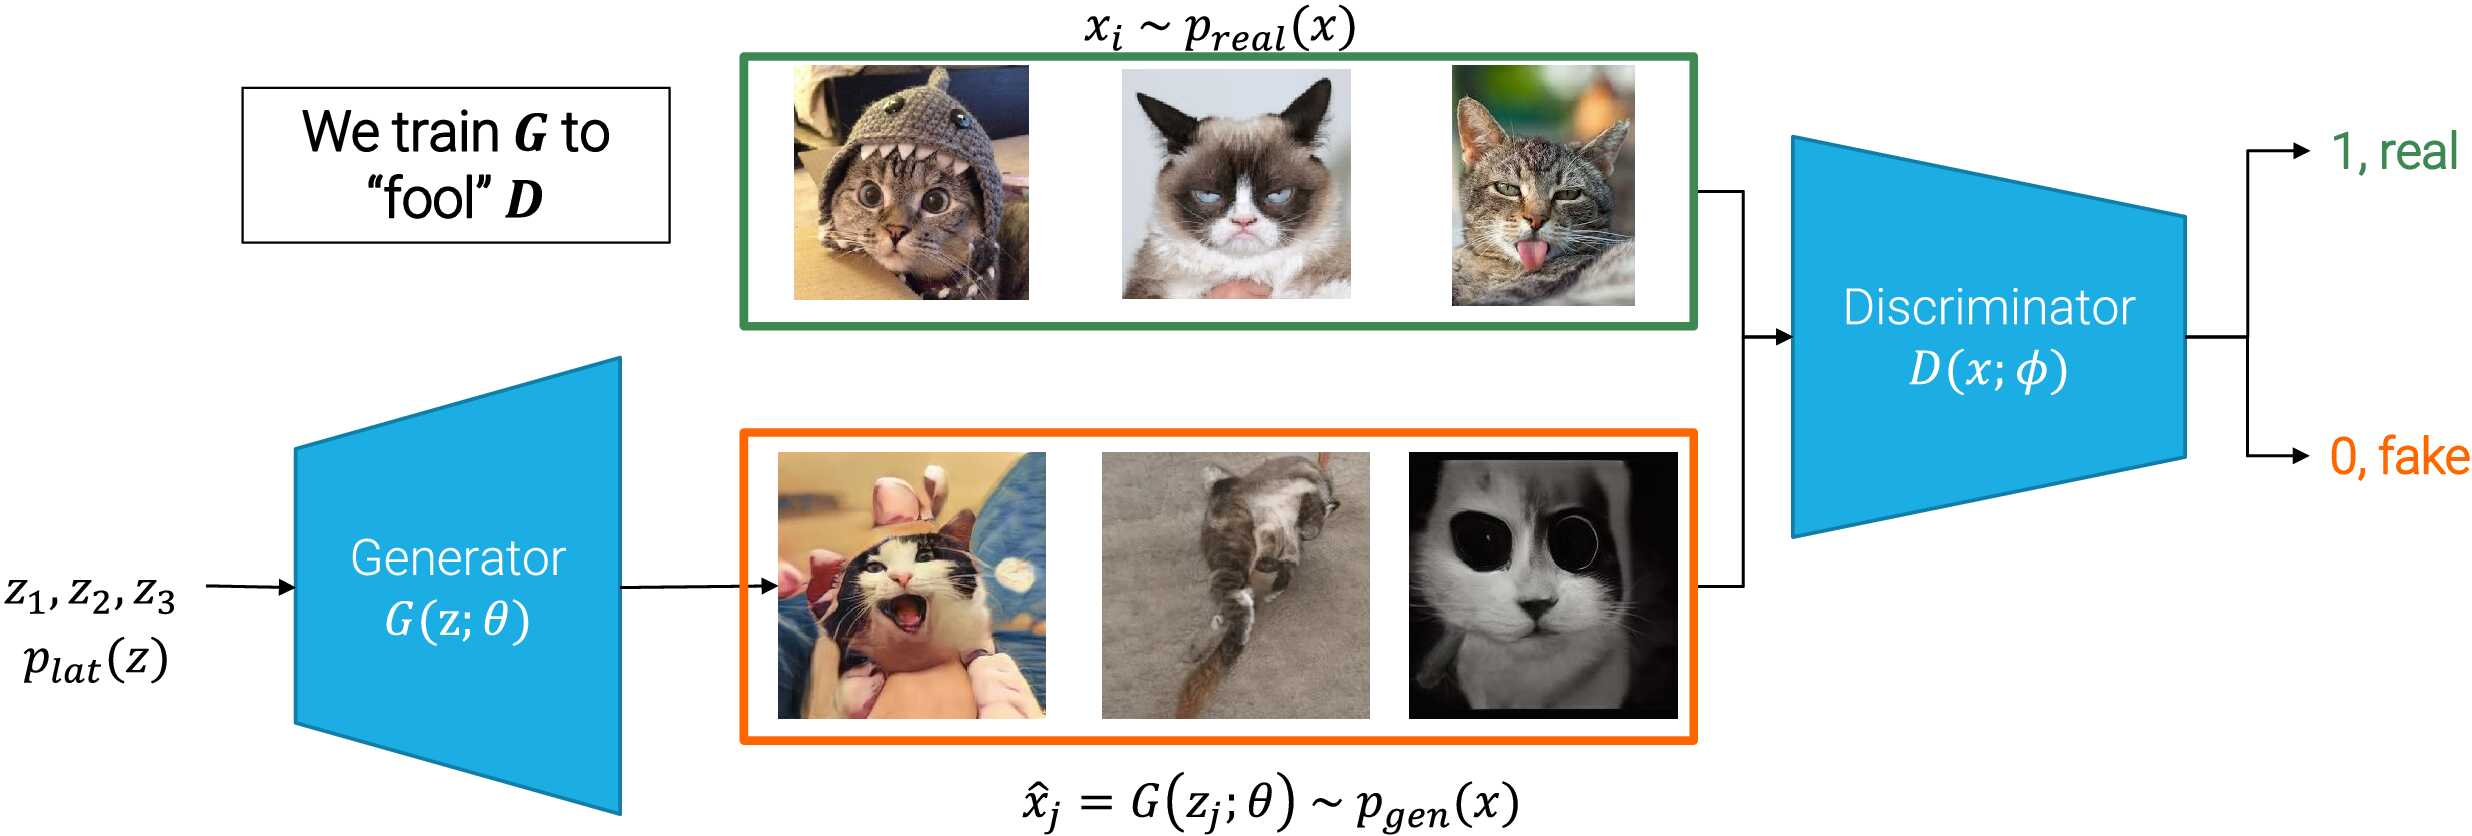
\includegraphics[width=0.8\linewidth]{./img/_gan_flow.jpg}
        \end{figure}


        \begin{description}
            \item[Discriminator loss] \marginnote{Discriminator loss}
                The discriminator solves a binary classification task using binary cross-entropy:
                \[ \mathcal{L}_\text{BCE}(\hat{y}, y) = -y \log(\hat{y}) - (1-y)\log(1-\hat{y}) \]
                As real images always have label $1$ and generated ones always $0$, the optimal parameters are given by the problem:
                \[ 
                    \begin{split}
                        \phi^* &= \arg\min_{\phi} \left\{ 
                            \frac{1}{I} \sum_{i=1}^I \mathcal{L}_\text{BCE}(D(x_i; \phi), 1) + 
                            \frac{1}{J} \sum_{j=1}^J \mathcal{L}_\text{BCE}(D(\hat{x}_j; \phi), 0) 
                        \right\} \\ 
                        &= \arg\min_{\phi} \left\{ 
                            -\frac{1}{I} \sum_{i=1}^I \log \left( D(x_i; \phi) \right) - 
                            \frac{1}{J} \sum_{j=1}^J \log \left( 1- D(\hat{x}_j; \phi) \right) 
                        \right\}
                    \end{split}
                \]
                Therefore, the discriminator loss can be formulated as:
                \[ \mathcal{L}_D(\phi) = - \sum_{i=1}^{I} \log(D(x_i; \phi)) - \sum_{j=1}^{J} \log(1-D(\hat{x}_i; \phi)) \]

            \item[Generator loss] \marginnote{Generator loss}
                The generator aims to fool the discriminator. Its objective is therefore to maximize the loss the discriminator is minimizing:
                \[ \theta^* = \arg\max_\theta \left\{ \min_{\phi} \left\{ 
                    -\frac{1}{I} \sum_{i=1}^I \log \left( D(x_i; \phi) \right) - 
                    \frac{1}{J} \sum_{j=1}^J \log \left( 1- D(G(z_j; \theta); \phi) \right) 
                \right\} \right\} \]
                As the generator only influences the second term, the overall generator loss is:
                \[ \mathcal{L}_G(\theta) = \sum_{j=1}^{J} \log\left( 1 - D(G(z_j; \theta); \phi) \right) \]


            \item[Training]
                Generator and discriminator are trained together in a minimax game as follows:
                \begin{enumerate}
                    \item Sample a batch of latent vectors $z_1, \dots, z_j$ to generate $\hat{x}_1, \dots, \hat{x}_j$.
                    \item Sample a batch of real images $x_1, \dots, x_i$.
                    \item Merge the two batches and optimize for $\mathcal{L}_D(\phi)$ and $\mathcal{L}_G(\theta)$.
                \end{enumerate}
        \end{description}

        \begin{remark}[Optimal discriminator]
            The discriminator loss can be seen as a sum of two expectations (that uses Monte Carlo approximation):
            \[ 
                \begin{split}
                    \mathcal{L}_D(\phi) &= - \frac{1}{I} \sum_{i=1}^{I} \log(D(x_i; \phi)) - \frac{1}{J} \sum_{j=1}^{J} \log(1-D(\hat{x}_i; \phi)) \\
                    &\approx -\mathbb{E}_{x_i \sim p_\text{real}(x)}\left[ \log(D(x_i; \phi)) \right] - \mathbb{E}_{\hat{x}_j \sim p_\text{gen}(x)}\left[ \log(1-D(\hat{x}_j; \phi)) \right] \\
                    &= - \int p_\text{real}(x) \log(D(x; \phi)) + p_\text{gen}(x) \log(1-D(x; \phi)) \,dx
                \end{split}
            \]
            By calling $a = p_\text{real}(x)$, $b = p_\text{gen}(x)$, and $y = D(x; \phi)$, we have that:
            \[ \int a \log(y) + b \log(1-y) \,dx \]
            To obtain the minimum w.r.t. $y = D(x; \phi)$, we have that:
            \[ 
                \begin{split}
                    \frac{\partial}{\partial y}\left[ a \log(y) + b \log(1-y) \right] = 0 
                    &\Rightarrow \frac{a}{y} - \frac{b}{1-y} = 0 \\
                    &\Rightarrow y = \frac{a}{a-b}
                \end{split}
            \]
            Therefore, the optimal theoretical discriminator is:
            \[ D^*(x) = \frac{p_\text{real}(x)}{p_\text{real}(x) + p_\text{gen}(x)} \]
            This makes sense as:
            \begin{itemize}
                \item With a real image ($p_\text{real}(x)$ high) and a bad generator ($p_\text{gen}(x)$ low), the discriminator is able to detect the real image ($D^*(x) \rightarrow 1$).
                \item With a bad generator ($p_\text{real}(x)$ low and $p_\text{gen}(x)$ high), the discriminator is able to detect the generator ($D^*(x) \rightarrow 0$).
                \item With a perfect generator ($p_\text{real}(x)$ and $p_\text{gen}(x)$ are both high), the discriminator is undecided ($D^*(x) \rightarrow 0.5$).
            \end{itemize}
        \end{remark}

        \begin{remark}[Optimal generator]
            By inserting the optimal discriminator into the (full) generator loss, we have that:
            \[
                \footnotesize
                \begin{split}
                    \mathcal{L}_G(x) &= - \int p_\text{real}(x) \log\left(\frac{p_\text{real}(x)}{p_\text{real}(x) + p_\text{gen}(x)}\right) + p_\text{gen}(x) \log\left(1 - \frac{p_\text{real}(x)}{p_\text{real}(x) + p_\text{gen}(x)}\right) \,dx \\
                    &= - \int p_\text{real}(x) \log\left(\frac{p_\text{real}(x)}{p_\text{real}(x) + p_\text{gen}(x)}\right) \,dx - \int p_\text{gen}(x) \log\left(\frac{p_\text{gen}(x)}{p_\text{real}(x) + p_\text{gen}(x)}\right) \,dx \\
                    &= - \int p_\text{real}(x) \log\left({\frac{2}{2}} \frac{p_\text{real}(x)}{p_\text{real}(x) + p_\text{gen}(x)}\right) \,dx - \int p_\text{gen}(x) \log\left({\frac{2}{2}} \frac{p_\text{gen}(x)}{p_\text{real}(x) + p_\text{gen}(x)}\right) \,dx \\
                    &= - \int p_\text{real}(x) \log\left(\frac{{2} p_\text{real}(x)}{p_\text{real}(x) + p_\text{gen}(x)}\right) + {\log\left(\frac{1}{2}\right)} \,dx - \int p_\text{gen}(x) \log\left(\frac{{2} p_\text{gen}(x)}{p_\text{real}(x) + p_\text{gen}(x)}\right) + {\log\left(\frac{1}{2}\right)} \,dx \\
                    &= - \int p_\text{real}(x) \log\left(\frac{2 p_\text{real}(x)}{p_\text{real}(x) + p_\text{gen}(x)}\right) \,dx - \int p_\text{gen}(x) \log\left(\frac{2 p_\text{gen}(x)}{p_\text{real}(x) + p_\text{gen}(x)}\right) \,dx + \log(4)  \\
                    &= - \int p_\text{real}(x) \log\left(\frac{p_\text{real}(x)}{\frac{p_\text{real}(x) + p_\text{gen}(x)}{2}}\right) \,dx - \int p_\text{gen}(x) \log\left(\frac{p_\text{gen}(x)}{\frac{p_\text{real}(x) + p_\text{gen}(x)}{2}}\right) \,dx + \log(4)  \\
                    &= - D_\text{KL}\left( p_\text{real}(x) || \frac{p_\text{real}(x) + p_\text{gen}(x)}{2} \right) - D_\text{KL}\left( p_\text{gen}(x) || \frac{p_\text{real}(x) + p_\text{gen}(x)}{2} \right) + \log(4) \\
                    &= -2 D_\text{JS}\left( p_\text{real}(x) || p_\text{gen}(x) \right) + \log(4)
                \end{split}
            \]
            Therefore, the generator aims to maximize $-2 D_\text{JS}\left( p_\text{real}(x) || p_\text{gen}(x) \right) + \log(4)$. As $D_\text{JS}(\cdot) \geq 0$, the optimal generator aims to achieve $D_\text{JS}(\cdot) = 0$ which happens when:
            \[ p_\text{real}(x) = p_\text{gen}(x) \]
        \end{remark}

        \begin{remark}
            Even though on a theoretical level a perfect discriminator and generator exist, in practice neural networks are finite and it is not clear if the alternating minimization steps converge.
        \end{remark}

        \begin{remark}
            The original GAN only uses fully-connected layers.
        \end{remark}
\end{description}


\subsection{Deep convolutional GAN}

\begin{description}
    \item[Deep convolutional GAN (DCGAN)] \marginnote{Deep convolutional GAN (DCGAN)}
        GAN with a fully-convolutional architecture.

        \begin{figure}[H]
            \centering
            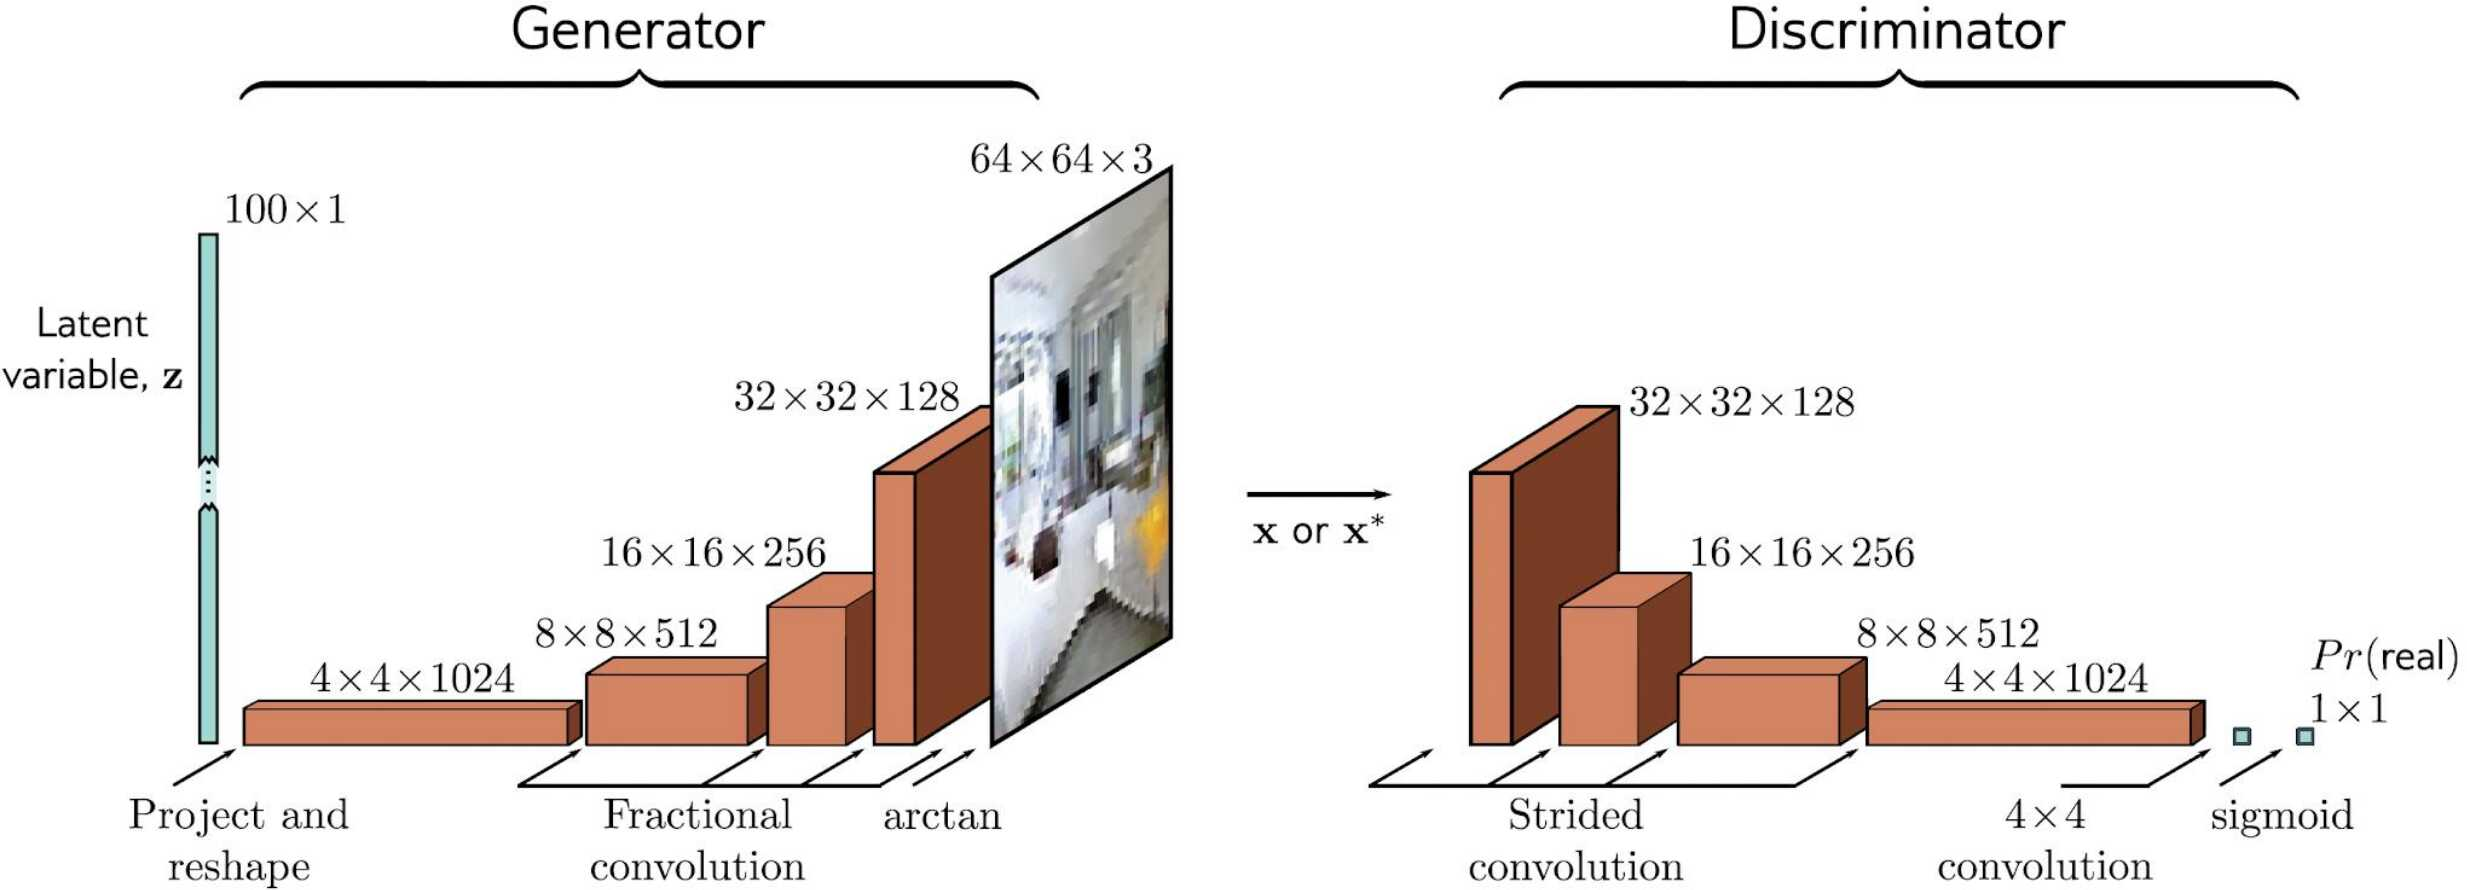
\includegraphics[width=0.6\linewidth]{./img/dcgan.jpg}
        \end{figure}
\end{description}

\begin{remark}
    The latent space of GANs is well-behaved: directions in the latent space have a meaning.

    \begin{figure}[H]
        \centering
        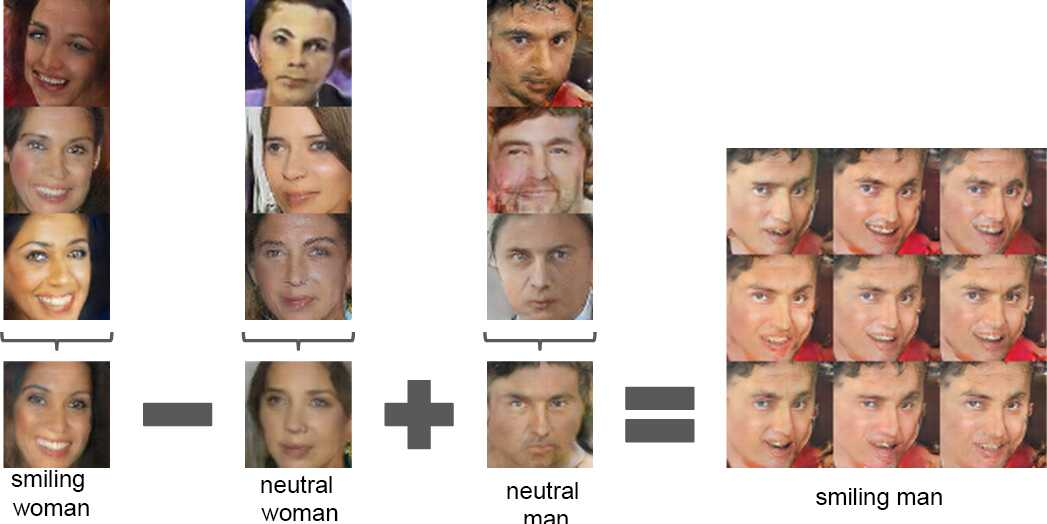
\includegraphics[width=0.5\linewidth]{./img/gan_latent_interpolation.jpg}
    \end{figure}
\end{remark}

\begin{remark}[Mode dropping/collapse]
    Only some modes of the distribution of the real data are represented by the mass of the generator.

    Consider the training objective of the optimal generator. The two terms model coverage and quality, respectively:
    \[ 
        \begin{gathered}
            -\frac{1}{I} \sum_{i=1}^I \log \left( D(x_i; \phi) \right) - \frac{1}{J} \sum_{j=1}^J \log \left( 1- D(G(z_j; \theta); \phi) \right) \\
            = - \underbrace{D_\text{KL}\left( p_\text{real}(x) || \frac{p_\text{real}(x) + p_\text{gen}(x)}{2} \right)}_{\text{Coverage}}
            - \underbrace{D_\text{KL}\left( p_\text{gen}(x) || \frac{p_\text{real}(x) + p_\text{gen}(x)}{2} \right)}_{\text{Quality}}
            + \log(4) 
        \end{gathered}
    \]
    The coverage term is high for regions with real images and no generated ones. The quality term is high for regions with generated images and no real ones.

    As the generator only affects the second term (quality), this might be a reason that causes mode collapse.
\end{remark}

\begin{remark}[Disjoint distributions]
    As real and generated images lie in low-dimensional subspaces, it is likely that their distributions are disjoint. The training objective of GANs aims to minimize the JS divergence, which is maximum if the distributions do not overlap causing no significant signal for gradient updates.

    In other words, whenever the generator or discriminator becomes too performant (i.e., the distributions become too different), updates to the other component carry no signal.

    \begin{figure}[H]
        \centering
        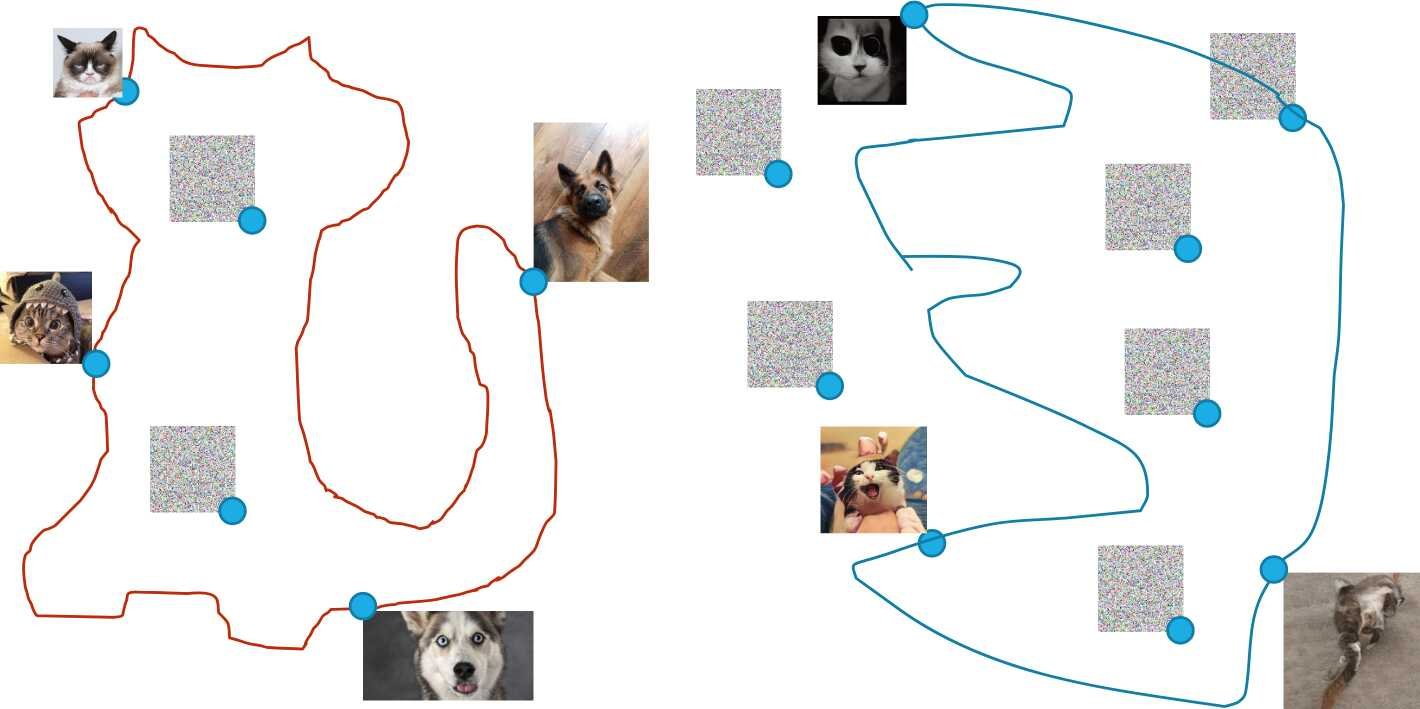
\includegraphics[width=0.7\linewidth]{./img/gan_disjoint.jpg}
    \end{figure}

    \indenttbox
    \begin{example}
        By freezing the generator while training the discriminator, it takes few epochs for it to achieve near perfect accuracy.
    \end{example}
\end{remark}


\subsection{Wasserstein GAN}

\begin{description}
    \item[Wasserstein GAN (WGAN)] \marginnote{Wasserstein GAN (WGAN)}
        Train a GAN using the Wasserstein distance (i.e., EMD) to compare distributions.

        \begin{remark}
            The Wasserstein distance is meaningful even with disjoint distributions.
        \end{remark}

        \begin{remark}
            It can be shown that the objective is easier to optimize in the dual form of the linear programming formulation.
        \end{remark}
\end{description}


\subsection{Progressive GAN}

\begin{description}
    \item[Progressive GAN (ProGAN)] \marginnote{Progressive GAN (ProGAN)}
        GAN for high-resolution generation with a coarse-to-fine approach. 
        
        \begin{description}
            \item[Training] 
                The network starts as a generator for $4 \times 4$ images and its resolution is incrementally increased.

                \begin{figure}[H]
                    \centering
                    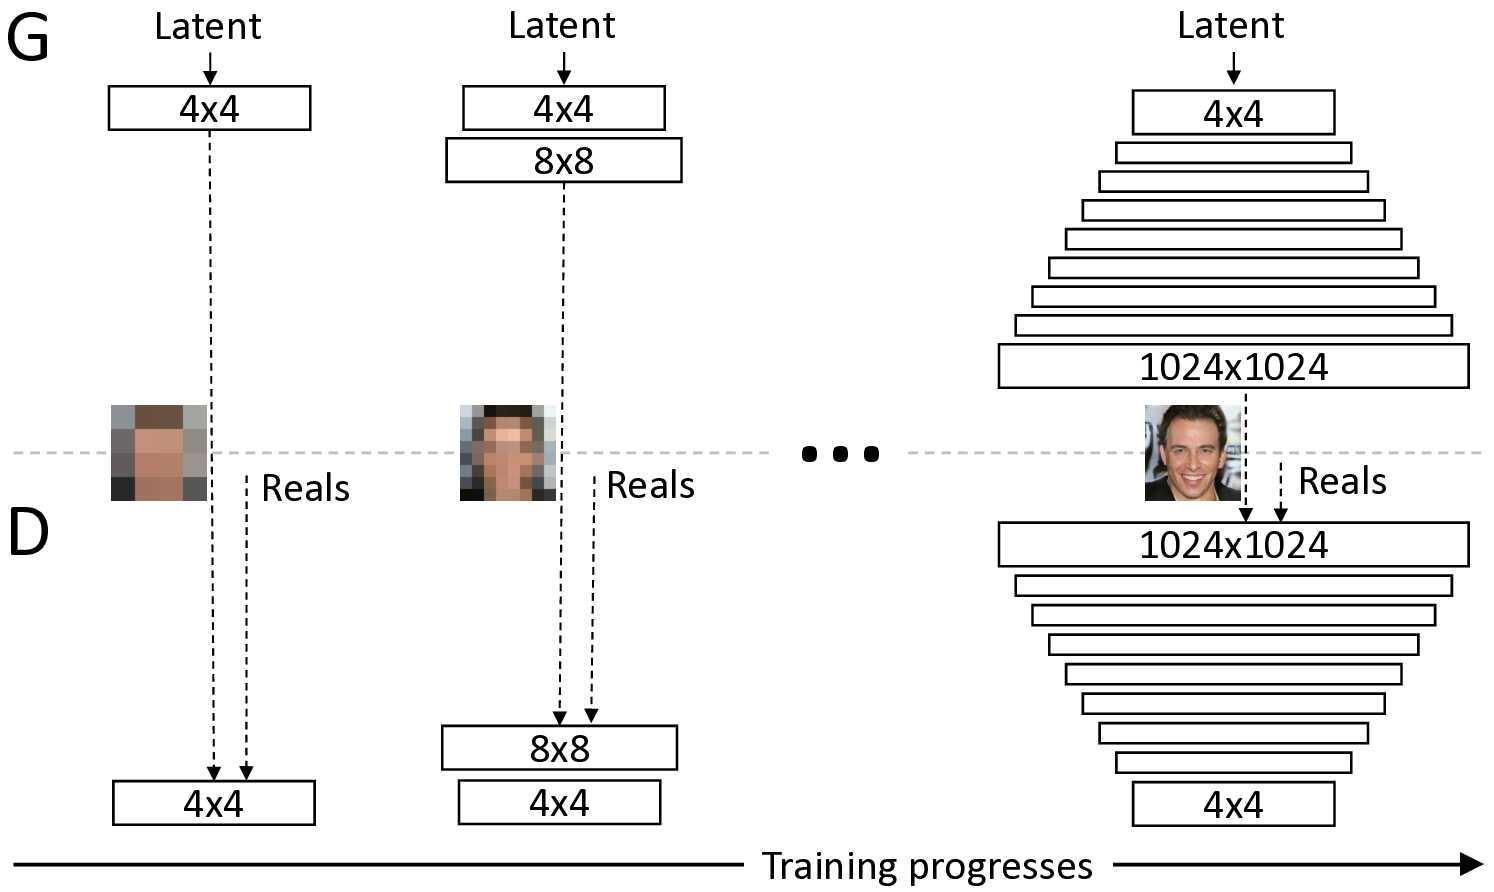
\includegraphics[width=0.65\linewidth]{./img/_progan.jpg}
                \end{figure}

                \begin{description}
                    \item[Layer fade-in] 
                        When moving from an $n \times n$ to $2n \times 2n$ resolution, the following happens:
                        \begin{itemize}
                            \item The generator outputs a linear combination between the $n \times n$ image up-sampled (with weight $1-\alpha$) and the $n \times n$ image passed through a transpose convolution (with weight $\alpha$).
                            \item The discriminator uses a linear combination between the $2n \times 2n$ image down-sampled (with weight $1-\alpha$) and the $2n \times 2n$ image passed through a convolution.
                        \end{itemize}
                        Where $\alpha$ grows linearly from 0 to 1 during training. This allows the network to use old information when the resolution changes and gradually adapt.

                        \begin{figure}[H]
                            \centering
                            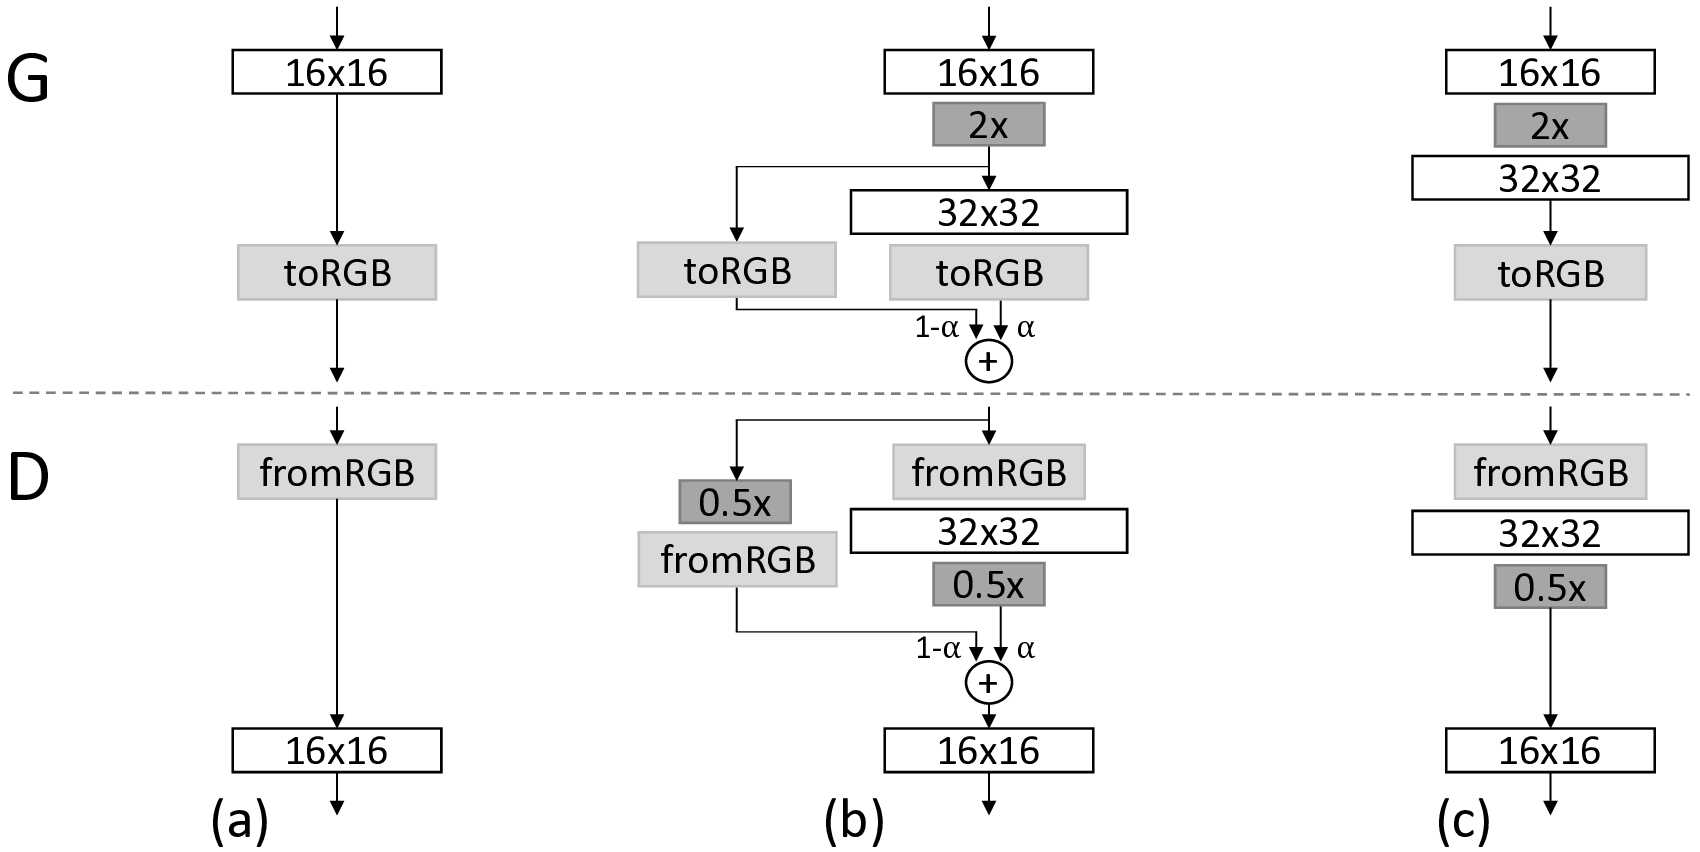
\includegraphics[width=0.7\linewidth]{./img/_progan_fadein.jpg}
                            \caption{
                                \parbox[t]{0.7\linewidth}{
                                    ProGAN fade-in. (a) is the starting resolution. (b) depicts the fade-in process. (c) represents the network at the end of the training process for this resolution (i.e., with $\alpha=1$)
                                }
                            }
                        \end{figure}
                \end{description}
        \end{description}
\end{description}


\subsection{StyleGAN}

\begin{description}
    \item[Instance normalization] \marginnote{Instance normalization}
        Normalize along spatial dimensions only (i.e., there is a mean and variance for every channel of the image and every element of the batch).

        \begin{description}
            \item[Adaptive instance normalization (AdaIN)] \marginnote{Adaptive instance normalization (AdaIN)}
                Given a content $c \in \mathbb{R}^{B \times C \times H \times W}$ and a style $s \in \mathbb{R}^{B \times C \times H \times W}$, AdaIN normalizes $c$ while injecting information from $s$ as follows:
                \[ \sqrt{v_s} \frac{c - \mu_c}{\sqrt{v_c + \varepsilon}} + \mu_s \]
                where $\mu_c \in \mathbb{R}^{B \times C \times 1 \times 1}$ and $v_c \in \mathbb{R}^{B \times C \times 1 \times 1}$ are mean and variance of $c$ and $\mu_s \in \mathbb{R}^{B \times C \times 1 \times 1}$ and $v_s \in \mathbb{R}^{B \times C \times 1 \times 1}$ are mean and variance of $s$.
        \end{description}


    \item[StyleGAN] \marginnote{StyleGAN}
        Network that does the following:
        \begin{enumerate}
            \item Preprocess the input latent vector with fully-connected layers.
            \item Add to the starting constant image (learned during training) some noise.
            \item Pass the current image as the content of AdaIN and use the refined latent vector as the style.
            \item Continue as normal GANs, with AdaIN using the latent vector as style after every convolution.
        \end{enumerate}

        \begin{figure}[H]
            \centering
            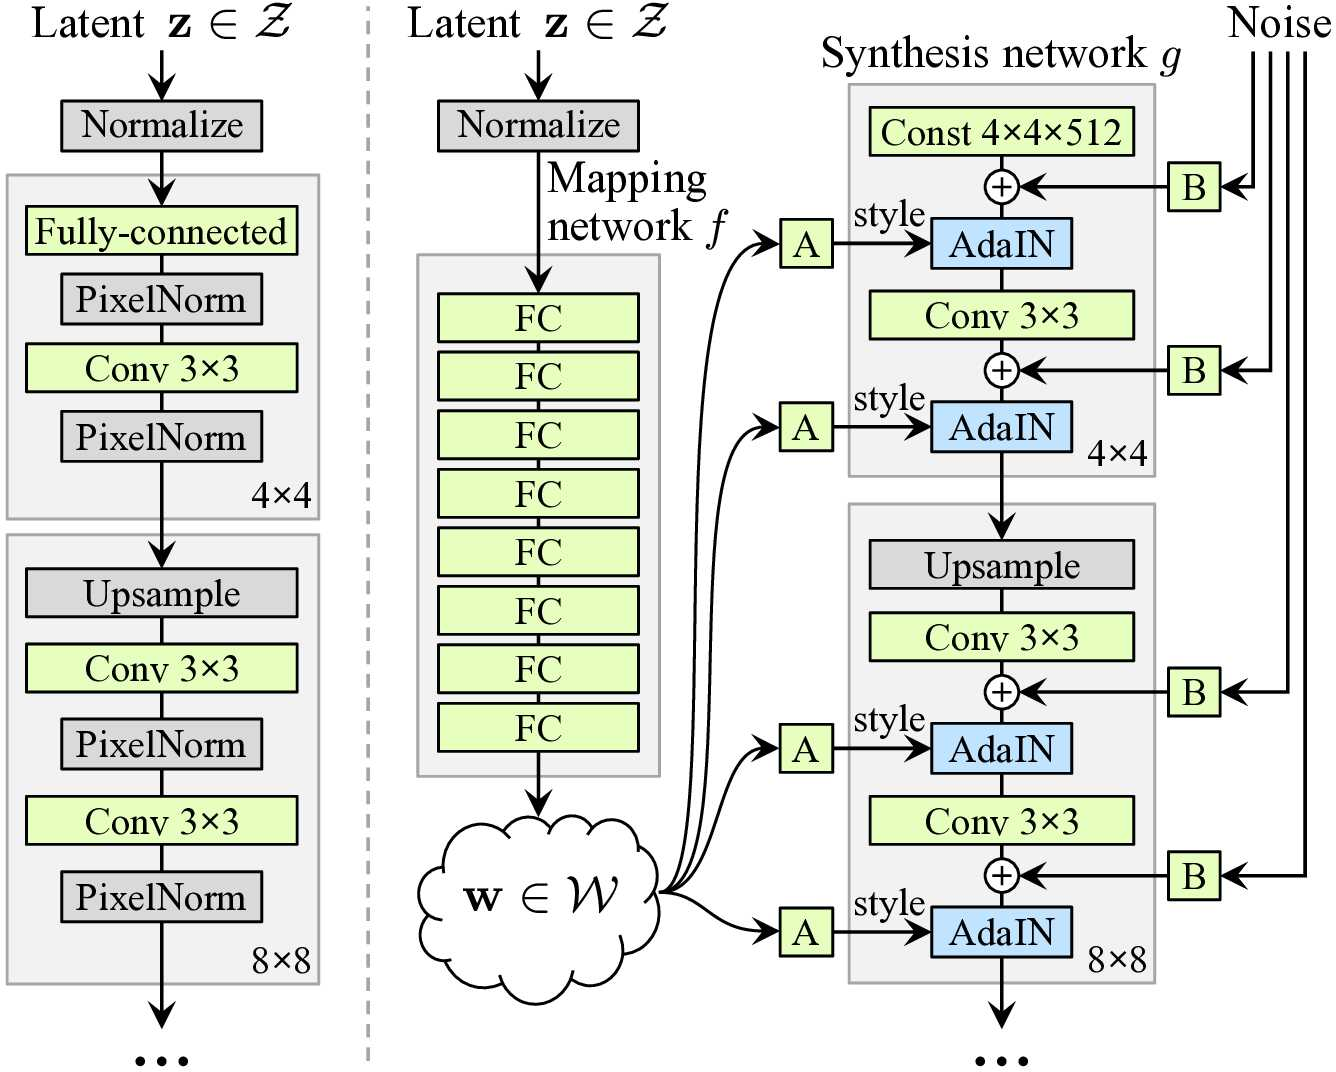
\includegraphics[width=0.4\linewidth]{./img/_stylegan.jpg}
        \end{figure}

        \begin{remark}
            It has been observed that the refined latent representation is more disentangled.
        \end{remark}

        \begin{remark}
            In normal GANs, the latent vector encodes both information on the image to generate and some noise for variability. In StyleGAN, these two aspects are ideally separated.
        \end{remark}
\end{description}

\begin{remark}
    Adversarial losses can also be used in supervised problems (e.g., generate a colored version of a black-and-white image).
\end{remark}

\begin{remark}[BigGAN] \marginnote{BigGAN}
    To improve realism (with loss in coverage), a latent can be sampled from only the high-probability areas of the distribution.
\end{remark}



\section{Diffusion models}

\def\x{\matr{x}}
\def\params{\matr{\theta}}
\def\noise{\matr{\varepsilon}}


\begin{description}
    \item[Diffusion model] \marginnote{Diffusion model}
        Architecture that generates an image by iteratively denoising the input latent vector.

        \begin{remark}
            Empirical results show that the generation quality is generally better than other models. However, inference is slow.
        \end{remark}

    \item[Training]
        Given an image $\x_0$, training is done in two steps:
        \begin{description}
            \item[Forward process] 
                The original image $\x_0$ is iteratively transformed into a latent image $\x_T$ by adding noise (i.e., transform the complex distribution $q(\x_0)$ of the original image into a simpler one $q(\x_T)$).
            \item[Reverse process] 
                The latent image $\x_T$ is iteratively denoised to reconstruct the original image $\x_0$.
        \end{description} 

        \begin{figure}[H]
            \centering
            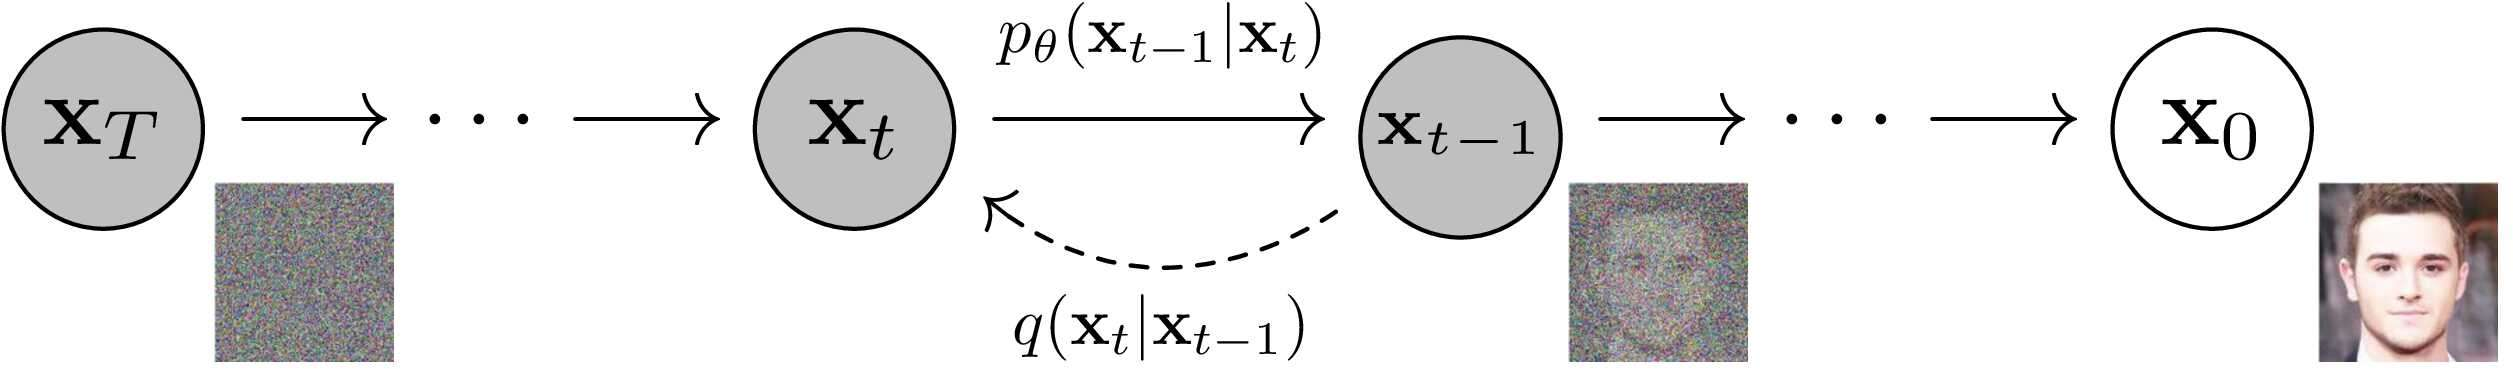
\includegraphics[width=0.8\linewidth]{./img/diffusion_model.jpg}
        \end{figure}
\end{description}


\subsection{Forward process}

\begin{description}
    \item[Forward process] \marginnote{Forward process}
        Given an image $\x_{t-1}$, produce a noisier version of it as:
        \[ 
            \begin{gathered}
                \x_t = \sqrt{1-\beta_t} \x_{t-1} + \sqrt{\beta_t}\noise_t \\
                \x_t \sim q(\x_t \mid \x_{t-1}) = \mathcal{N}(\sqrt{1-\beta_t}\x_{t-1}; \beta_t\matr{I})
            \end{gathered}
        \]
        where:
        \begin{itemize}
            \item $\noise_t \sim \mathcal{N}(0; \matr{I})$ is the noise
            \item $\beta_t \in [0,1)$ is a hyperparameter (noise schedule) and represents the variance.
            \item $\sqrt{1-\beta_t} \x_{t-1}$ is the mean.
        \end{itemize}

        \begin{remark}
            $\sqrt{1-\beta_t} \x_{t-1}$ and $\beta_t$ are the mean and variance due to the fact that sampling a vector $\vec{x}$ from a Gaussian distribution with mean $\vec{\mu}$ and covariance matrix $\matr{\Sigma}$ is equivalent to:
            \[ \vec{x} = \vec{\mu} + \matr{\Sigma}^{\frac{1}{2}}\vec{y} \qquad \text{where } \vec{y} \sim \mathcal{N}(0; \matr{I}) \]
            If $\matr{\Sigma} = \sigma^2\matr{I}$, it holds that $\matr{\Sigma}^{\frac{1}{2}} = \sigma \matr{I}$ and we have that:
            \[ \vec{x} = \vec{\mu} + (\sigma\matr{I})\vec{y} \]
        \end{remark}

        \begin{remark}
            This step does not have learnable parameters.
        \end{remark}

    \item[Diffusion kernel] \marginnote{Diffusion kernel}
        It is possible to generate the latent vector $\x_t$ at time $t$ directly from $\x_0$ as:
        \[ \x_t = \sqrt{\prod_{i=1}^{t}(1-\beta_i)} \cdot \x_0 + \sqrt{1-\prod_{i=1}^{t}(1-\beta_i)} \cdot \noise \qquad \text{where } \noise \sim \mathcal{N}(0; \matr{I}) \]
        By setting the intermediate constant $\alpha_t = \prod_{i=1}^{t}(1-\beta_i)$, we have that:
        \[ 
            \begin{gathered}
                \x_t = \sqrt{\alpha_t} \x_0 + \sqrt{1-\alpha_t}\noise \\
                \x_t \sim q(\x_t \mid \x_0) = \mathcal{N}(\sqrt{\alpha_t}\x_0; (1-\alpha_t)\matr{I})
            \end{gathered}
        \]

        \begin{remark}
            As $\beta_t < 1$, it holds that $\lim\limits_{t \rightarrow +\infty} \alpha_t = 0$. In other words, for large $t = T$, only noise remains in the latent vector:
            \[ q(\x_T \mid \x_0) = q(\x_T) = \mathcal{N}(0; \matr{I}) \]
            Which achieves the goal of transforming a complex distribution $q(\x_0)$ into a simpler one (i.e., Gaussian).
        \end{remark}

        \begin{example}
            Consider the 1D case where $x$ represents a pixel. By using a linear scheduling for $\beta_t$ as follows:
            \begin{figure}[H]
                \centering
                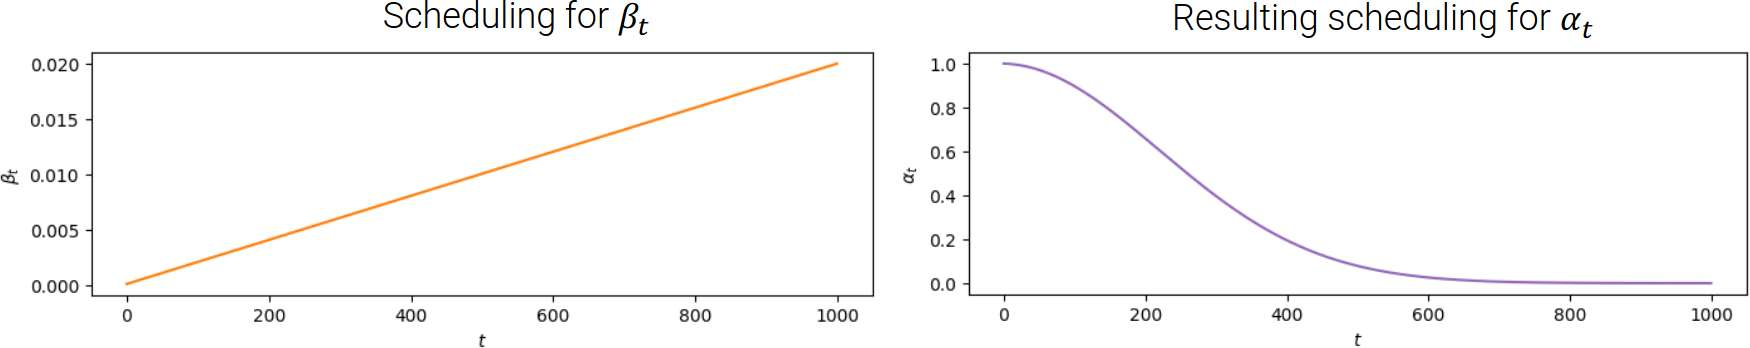
\includegraphics[width=0.9\linewidth]{./img/diffusion_kernel_example1.jpg}
            \end{figure}
            We obtain that some diffusion kernels for varying $t$ with $x_0 = 1$ are the following (note that the signal converges to $\mathcal{N}(0; 1)$):
            \begin{figure}[H]
                \centering
                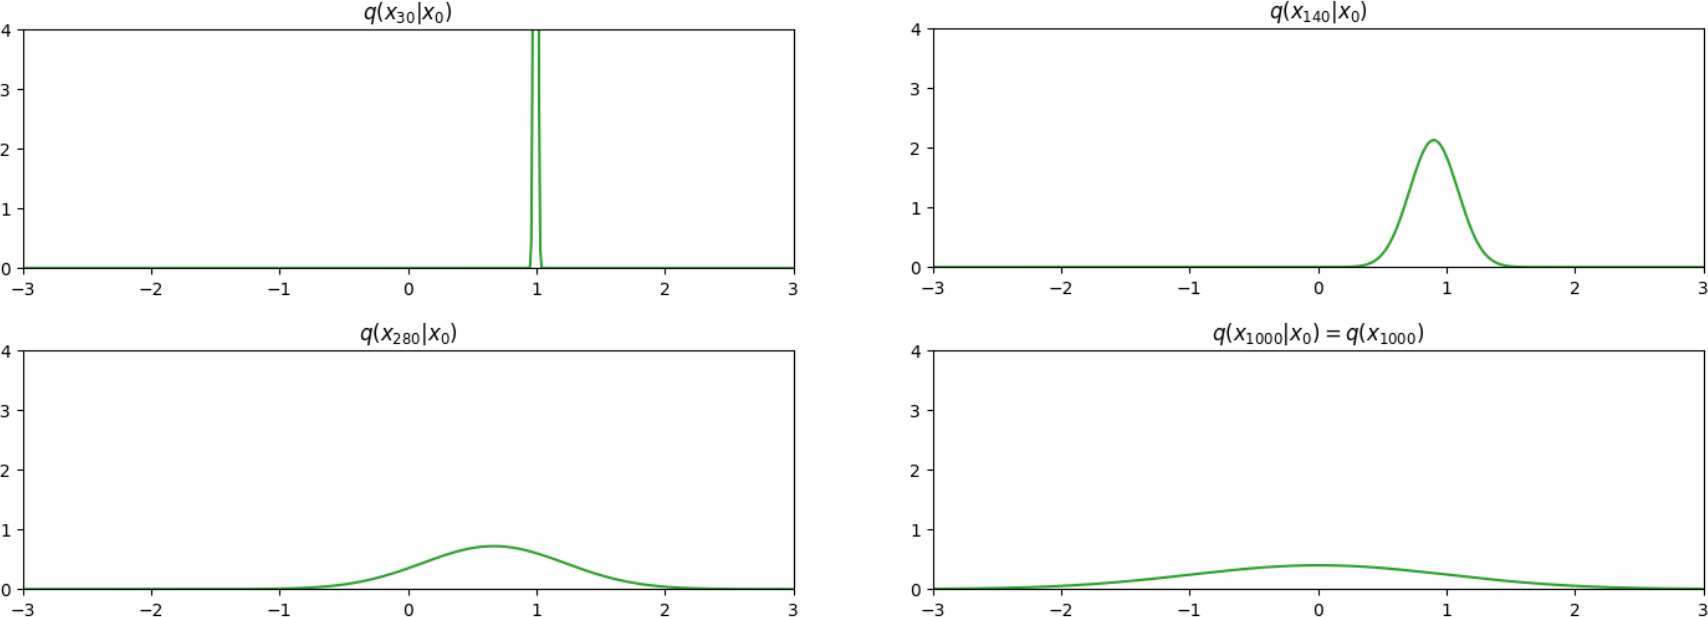
\includegraphics[width=0.9\linewidth]{./img/diffusion_kernel_example2.jpg}
            \end{figure}
        \end{example}

        \begin{remark}
            As the forward process is stochastic, the same starting pixel can produce a different resulting pixel. Therefore, diffusion models work with trajectories in latent space.

            \begin{figure}[H]
                \centering
                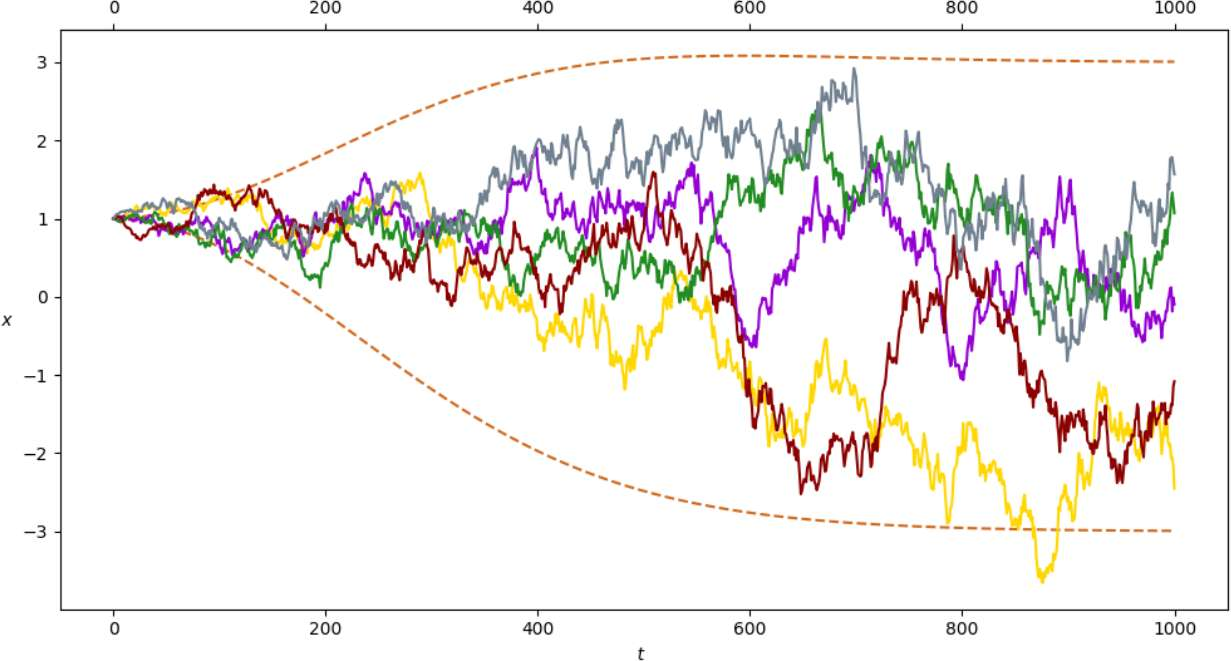
\includegraphics[width=0.6\linewidth]{./img/diffusion_model_trajectory.jpg}
                \caption{
                    \parbox[t]{0.6\linewidth}{
                        Trajectories starting from $x_0 = 1$. The dashed lines mark the $\mu_t \pm 3\sigma_t$ area.
                    }
                }
            \end{figure}
        \end{remark}
\end{description}


\subsection{Reverse process}

\begin{remark}
    In principle, one could invert the forward process by applying Bayes' rule:
    \[ q(\x_{t-1} \mid \x_t) = q(\x_t \mid \x_{t-1}) \frac{q(\x_{t-1})}{q(\x_t)} \]
    However, closed-form expressions for $q(\x_{t-1})$ and $q(\x_{t})$ are not available.

    By exploiting the Markov chain properties, it is possible to compute the conditional distribution w.r.t. $\x_0$, which is available at training time, as:
    \[ 
        q(\x_{t-1} \mid \x_t, \x_0) = 
        q(\x_t \mid \x_{t-1}, \x_0) \frac{q(\x_{t-1} \mid \x_0)}{q(\x_t \mid \x_0)} = 
        \underbrace{{q(\x_t \mid \x_{t-1})}}_{\text{Forward process}}
        \underbrace{\frac{q(\x_{t-1} \mid \x_0)}{q(\x_t \mid \x_0)}}_{\text{Diffusion kernels}}
    \]
    It can be shown that this is equivalent to:
    \[ q(\x_{t-1} \mid \x_t, \x_0) = \mathcal{N}\left( \frac{1-\alpha_{t-1}}{1-\alpha_t}\sqrt{1-\beta_t}\x_t + \frac{\sqrt{\alpha_{t-1}}}{1-\alpha_t}\beta_t \x_0; \frac{\beta_t(1-\alpha_{t-1})}{1-\alpha_t} \matr{I} \right) \]
    However, this formulation requires knowing $\x_0$, which is only available at training time, making inference impossible.
\end{remark}

\begin{description}
    \item[Learned reverse process (mean)] \marginnote{Learned reverse process (mean)}
        Learn a Markov chain of probabilistic mappings to reconstruct the original image $\x_0$ starting from the latent vector $\x_T$:
        \[
            \begin{split}
                p(\x_T) &= \mathcal{N}(0; \matr{I}) = q(\x_T) \\
                p(\x_{t-1} \mid \x_t) &= \mathcal{N}(\mu_t(\x_t; \params_t); \sigma_t\matr{I})
            \end{split}
        \]
        where:
        \begin{itemize}
            \item $\mu_t(\x_t; \params_t)$ is a neural network to estimate the mean of $p(\x_{t-1} \mid \x_t)$.
            \item $\sigma_t$ is, for the case of simple diffusion models, predetermined.
        \end{itemize}

        \begin{remark}
            In general, $p(\x_{t-1} \mid \x_t)$ does not necessarily follow a Gaussian distribution as this is only true for $\beta_t \rightarrow 0$. However, by using small $\beta_t$ and large $T$, it can be approximately considered Gaussian.
        \end{remark}

        \begin{description}
            \item[Loss]
                The loss function for a set of images $\{ \x_0^{(i)} \}_{i=1}^{I}$ is based on the MSE of the predicted means:
                \[ 
                    \small
                    \begin{split}
                        &\mathcal{L}(\params_1, \dots, \params_T) \\
                        &= \sum_{i=1}^{I}\Bigg( 
                            -\log\left( \mathcal{N}(\x_0^{(i)}; \mu_1(\x_1^{(i)}; \params_1), \sigma_1\matr{I}) \right) +
                            \sum_{t=2}^{T} \frac{1}{2\sigma_t} \bigg\Vert 
                                \matr{\mu}_{q(x_{t-1} \mid x_t, x_0)} -
                                \mu_t(\x_t^{(i)}; \matr{\theta_t}) \vphantom{\frac{\sqrt{0_0}}{0_0}}
                            \bigg\Vert^2
                        \Bigg) \\
                        &= \sum_{i=1}^{I}\Bigg( 
                            \underbrace{-\log\left( \mathcal{N}(\x_0^{(i)}; \mu_1(\x_1^{(i)}; \params_1), \sigma_1\matr{I}) \right)}_{\text{Reconstruction of $x_0$ from $x_1$}} +
                            \sum_{t=2}^{T} \frac{1}{2\sigma_t} \bigg\Vert 
                                \underbrace{\frac{1-\alpha_{t-1}}{1-\alpha_t} \sqrt{1-\beta_t} \x_t^{(i)} + \frac{\sqrt{\alpha_{t-1}}}{1-\alpha_t}\beta_t\x_0^{(i)}}_{\text{Ground-truth mean of $q(x_{t-1} \mid x_t, x_0)$}} -
                                \underbrace{\mu_t(\x_t^{(i)}; \matr{\theta_t}) \vphantom{\frac{\sqrt{0_0}}{0_0}}}_{\text{Prediction}}
                            \bigg\Vert^2
                        \Bigg)
                    \end{split}
                \]

                \begin{remark}
                    As $T$ is usually large, the MSE term has more relevance.
                \end{remark}

                \begin{marginbar}{darkgray}{0}{thick}
                \begin{proof}
                    The overall training objective for a set of real images $\{ \x_0^{(i)} \}_{i=1}^{I}$ is to maximize the likelihood of the reconstructed image:
                    \[ \params_1^*, \dots, \params_T^* = \arg\max_{\params_1, \dots, \params_T} \sum_{i=1}^{I} \log\left( p(\x_0^{(i)} \mid \params_1, \dots, \params_T) \right) \]

                    \indenttbox
                    \begin{marginbar}{darkgray}{0}{thick}
                    \begin{lemma}[Latents joint probabilites] \label{th:latents_joint}
                        As each image is obtained as a sequence of latents, we have that:
                        \begin{equation}
                            \begin{aligned}
                                p&(\x_0, \x_1, \dots, \x_T \mid \params_1, \dots, \params_T) \\
                                &= p(\x_0 \mid \x_1, \dots, \x_T, \params_1, \dots, \params_T) p(\x_1, \dots, \x_T \mid \params_1, \dots, \params_T) 
                                    & \text{\small $p(x, y | z) = p(x | y, z)p(y | z)$} \\
                                &= p(\x_0 \mid \x_1, \params_1) p(\x_1, \dots, \x_T \mid \params_2, \dots, \params_T) 
                                    & {\text{\small Markov chain}} \\
                                &= \dots & {\text{\small Repeat}} \\
                                &= p(\x_0 \mid \x_1, \params_1) \left( \prod_{t=2}^{T} p(\x_{t-1} \mid \x_t, \params_t) \right) p(\x_T)
                            \end{aligned}
                        \end{equation}
                    \end{lemma}
                    \end{marginbar}

                    By using \Cref{th:latents_joint}, the likelihood of $\x_0$ can be computed through marginalization over the latent images as follows:
                    \[ p(\x_0^{(i)} \mid \params_1, \dots, \params_T) = \int p(\x_0, \x_1, \dots, \x_T \mid \params_1, \dots, \params_T) \, d\x_1 \dots d\x_T \]
                    However, in practice this approach is computationally intractable due to the high number and high dimensionality of the latent variables.

                    \indenttbox
                    \begin{marginbar}{darkgray}{0}{thick}
                    \begin{lemma}[Jensen's inequality]
                        Given a concave function $f(\cdot)$ and the expectation of the data $x$. It holds that:
                        \[ f(\mathbb{E}_{x \sim p(x)}[x]) \geq \mathbb{E}_{x \sim p(x)}[f(x)] \]

                        \indenttbox
                        \begin{example}
                            Consider the logarithm function and a discrete random variable. It holds that:
                            \[ \log\left( \mathbb{E}_{x \sim p(x)}[x] \right) \geq \mathbb{E}_{x \sim p(x)}[\log(x)] \Rightarrow \log\left( \sum_{x \in \mathbb{X}} p(x)x \right) \geq \sum_{x \in \mathbb{X}} (p(x)\log(x)) \]
                        \end{example}

                        \begin{figure}[H]
                            \centering
                            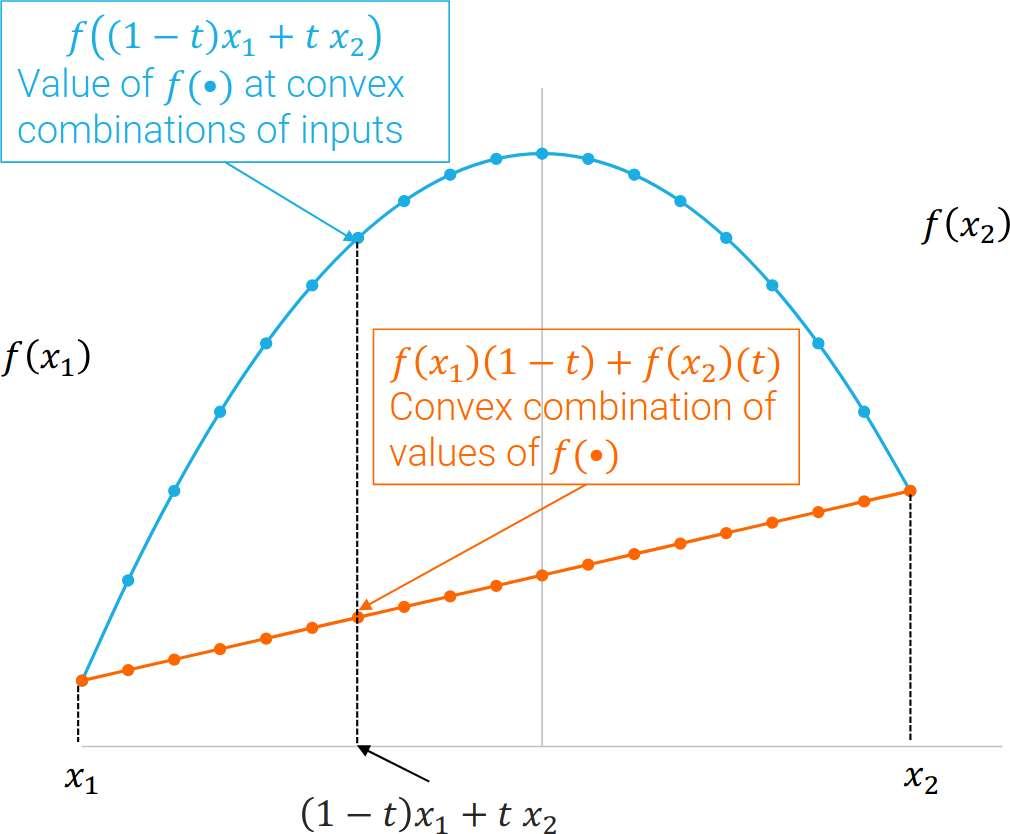
\includegraphics[width=0.45\linewidth]{./img/jensen_inequality.jpg}
                            \caption{Visualization of Jensen's inequality}
                        \end{figure}
                    \end{lemma}
                    \end{marginbar}

                    \indenttbox
                    \begin{marginbar}{darkgray}{0}{thick}
                    \begin{lemma}[Evidence lower bound (ELBO)] \marginnote{Evidence lower bound (ELBO)}
                        Method to compute a lower-bound of the log-likelihood. It holds that:
                        \[ 
                            \begin{split}
                                \log&(p(\x_0 \mid \params_1, \dots, \params_T)) \\ 
                                &= \log\left( \int p(\x_0, \x_1, \dots, \x_T \mid \params_1, \dots, \params_T) \, d\x_1 \dots d\x_T \right) \\
                                &= \log\left( \int \frac{q(\x_1, \dots, \x_T \mid \x_0)}{q(\x_1, \dots, \x_T \mid \x_0)} p(\x_0, \x_1, \dots, \x_T \mid \params_1, \dots, \params_T) \, d\x_1 \dots d\x_T \right) \\
                                &= \log\left( \mathbb{E}_{q(\x_1, \dots, \x_T \mid \x_0)}\left[ \frac{p(\x_0, \x_1, \dots, \x_T \mid \params_1, \dots, \params_T)}{q(\x_1, \dots, \x_T \mid \x_0)} \right] \right) \\
                            \end{split}
                        \]
                        By applying Jensen's inequality, ELBO is computed as:
                        \[
                            \begin{split}
                                \log&\left( \mathbb{E}_{q(\x_1, \dots, \x_T \mid \x_0)}\left[ \frac{p(\x_0, \x_1, \dots, \x_T \mid \params_1, \dots, \params_T)}{q(\x_1, \dots, \x_T \mid \x_0)} \right] \right) \geq \\
                                &\mathbb{E}_{q(\x_1, \dots, \x_T \mid \x_0)}\left[ \log\left( \frac{p(\x_0, \x_1, \dots, \x_T \mid \params_1, \dots, \params_T)}{q(\x_1, \dots, \x_T \mid \x_0)} \right) \right] = \texttt{ELBO}(\params_1, \dots, \params_T)
                            \end{split}
                        \]
                    \end{lemma}
                    \end{marginbar}

                    During training, we aim to maximize ELBO as a proxy to maximize the likelihood. By applying \Cref{th:latents_joint} to the argument of the logarithm in ELBO, we have that:
                    \[
                        \begin{aligned}
                            &\log\left( \frac{p(\x_0, \x_1, \dots, \x_T \mid \params_1, \dots, \params_T)}{q(\x_1, \dots, \x_T \mid \x_0)} \right) \\
                            &= \log\left( \frac{p(\x_0 \mid \x_1, \params_1) \left( \prod_{t=2}^{T} p(\x_{t-1} \mid \x_t, \params_t) \right) p(\x_T)}{q(\x_1 \mid \x_0) \prod_{t=2}^T q(\x_t \mid \x_{t-1}, \x_0)} \right) \\
                            &= \log\left( \frac{p(\x_0 \mid \x_1, \params_1)}{q(\x_1 \mid \x_0)} \right) + \log\left( \frac{\prod_{t=2}^{T} p(\x_{t-1} \mid \x_t, \params_t)}{\prod_{t=2}^T q(\x_t \mid \x_{t-1}, \x_0)} \right) + \log(p(\x_T)) \\
                            &= \log\left( \frac{p(\x_0 \mid \x_1, \params_1)}{q(\x_1 \mid \x_0)} \right) + \log\left( \prod_{t=2}^{T} \left( \frac{p(\x_{t-1} \mid \x_t, \params_t)}{q(\x_{t-1} \mid \x_{t}, \x_0)} \frac{q(\x_{t-1} \mid \x_0)}{q(\x_t \mid \x_0)} \right) \right) + \log(p(\x_T)) 
                                & \text{\small Bayes on denom.} \\
                        \end{aligned}
                    \]
                    The second term introduced by Bayes' rule can be simplified as follows:
                    \[
                        \begin{aligned}
                            \prod_{t=2}^T \frac{q(\x_{t-1} \mid \x_0)}{q(\x_t \mid \x_0)} &= \frac{q(\x_1 \mid \x_0)}{\cancel{q(\x_2 \mid \x_0)}} \frac{\cancel{q(\x_2 \mid \x_0)}}{\cancel{q(\x_3 \mid \x_0)}} \cdots \frac{\cancel{q(\x_{T-1} \mid \x_0)}}{q(\x_T \mid \x_0)} \\
                            &= \frac{q(\x_1 \mid \x_0)}{q(\x_T \mid \x_0)} \\
                            &= \frac{q(\x_1 \mid \x_0)}{q(\x_T)} & \text{\parbox{0.2\linewidth}{\small Time $T$ is known to be $\mathcal{N}(0; \matr{I})$}}
                        \end{aligned}
                    \]
                    Therefore, we have that:
                    \[
                        \begin{aligned}
                            &\log\left( \frac{p(\x_0 \mid \x_1, \params_1)}{\cancel{q(\x_1 \mid \x_0)}} \right) + \log\left( \frac{\cancel{q(\x_1 \mid \x_0)}}{q(\x_T)} \prod_{t=2}^{T} \frac{p(\x_{t-1} \mid \x_t, \params_t)}{q(\x_{t-1} \mid \x_{t}, \x_0)} \right) + \log(p(\x_T)) \\
                            &= \log\left( p(\x_0 \mid \x_1, \params_1) \right) + \log\left(\prod_{t=2}^{T} \frac{p(\x_{t-1} \mid \x_t, \params_t)}{q(\x_{t-1} \mid \x_{t}, \x_0)} \right) + \log\left( \frac{p(\x_T)}{q(\x_T)} \right) 
                                & \text{\parbox{0.29\linewidth}{\small $\frac{p(\x_T)}{q(\x_T)} \approx 1$ as they are both $\mathcal{N}(0; \matr{I})$}} \\
                            &= \log\left( p(\x_0 \mid \x_1, \params_1) \right) + \sum_{t=2}^{T} \log\left(\frac{p(\x_{t-1} \mid \x_t, \params_t)}{q(\x_{t-1} \mid \x_{t}, \x_0)} \right)
                        \end{aligned}
                    \]

                    By going back to ELBO, we have that:
                    \[
                        \small
                        \begin{aligned}
                            &\texttt{ELBO}(\params_1, \dots, \params_T) = \mathbb{E}_{q(\x_1, \dots, \x_T \mid \x_0)}\left[ \log\left( \frac{p(\x_0, \x_1, \dots, \x_T \mid \params_1, \dots, \params_T)}{q(\x_1, \dots, \x_T \mid \x_0)} \right) \right] \\
                            &\approx \mathbb{E}_{q(\x_1, \dots, \x_T \mid \x_0)}\left[ \log\left( p(\x_0 \mid \x_1, \params_1) \right) + \sum_{t=2}^{T} \log\left(\frac{p(\x_{t-1} \mid \x_t, \params_t)}{q(\x_{t-1} \mid \x_{t}, \x_0)} \right) \right] \\
                            &= \mathbb{E}_{q(\x_1 \mid \x_0)}\left[ \log\left( p(\x_0 \mid \x_1, \params_1) \right) \right] - \sum_{t=2}^{T} \mathbb{E}_{q(\x_1, \dots, \x_T \mid \x_0)}\left[ \log\left(\frac{q(\x_{t-1} \mid \x_{t}, \x_0)}{p(\x_{t-1} \mid \x_t, \params_t)} \right) \right] \\
                            & & \hspace{-2.5cm}\text{\small $\mathbb{E}_{q(x, y)} = \mathbb{E}_{q(y)} \mathbb{E}_{q(x \mid y)}$} \\
                            &= \mathbb{E}_{q(\x_1 \mid \x_0)}\left[ \log\left( p(\x_0 \mid \x_1, \params_1) \right) \right] - \sum_{t=2}^{T} \mathbb{E}_{q(\x_t \mid \x_0)}\mathbb{E}_{q(\x_1, \dots, \x_{t-1}, \x_{t+1}, \dots, \x_T \mid \x_t, \x_0)}\left[ \log\left(\frac{q(\x_{t-1} \mid \x_{t}, \x_0)}{p(\x_{t-1} \mid \x_t, \params_t)} \right) \right] \\
                            &= \mathbb{E}_{q(\x_1 \mid \x_0)}\left[ \log\left( p(\x_0 \mid \x_1, \params_1) \right) \right] - \sum_{t=2}^{T} \mathbb{E}_{q(\x_t \mid \x_0)}\mathbb{E}_{q(\x_{t-1} \mid \x_t, \x_0)}\left[ \log\left(\frac{q(\x_{t-1} \mid \x_{t}, \x_0)}{p(\x_{t-1} \mid \x_t, \params_t)} \right) \right] \\
                            &= \mathbb{E}_{q(\x_1 \mid \x_0)}\left[ \log\left( p(\x_0 \mid \x_1, \params_1) \right) \right] - \sum_{t=2}^{T} \mathbb{E}_{q(\x_t \mid \x_0)}\Big[ D_\text{KL}\big(q(\x_{t-1} \mid \x_t, \x_0) \Vert p(\x_{t-1} \mid \x_t, \params_t)\big) \Big] \\
                        \end{aligned}
                    \]

                    To make ELBO a computable loss function, we have to:
                    \begin{itemize}
                        \item Approximate expectations with Monte Carlo.
                        \item Expand $p$ and $q$ with their definition. 
                        \item Expand the KL divergence. As it is between two Gaussians with constant covariance matrices, it can be computed in closed form as:
                        \[ 
                            \begin{split}
                                D_\text{KL}&\big(q(\x_{t-1} \mid \x_t, \x_0) \Vert p(\x_{t-1} \mid \x_t, \params_t)\big) \\
                                &= \frac{1}{2\sigma_t} \left\Vert \matr{\mu}_{q(\x_{t-1} \mid \x_t, \x_0)} - \matr{\mu}_{p(\x_{t-1} \mid \x_t, \params_t)} \right\Vert^2 + c \\
                                &= \frac{1}{2\sigma_t} \left\Vert \left(\frac{1-\alpha_{t-1}}{1-\alpha_t} \sqrt{1-\beta_t} \x_t + \frac{\sqrt{\alpha_{t-1}}}{1-\alpha_t} \beta_t \x_0\right) - \mu_t(\x_t; \params_t) \right\Vert^2 + c
                            \end{split}
                        \]
                        where $c$ is a constant.
                    \end{itemize}

                    Finally, the loss is defined from ELBO as:
                    \[
                        \small
                        - \sum_{i=1}^{I}\Bigg( 
                            \log\left( \mathcal{N}(\x_0^{(i)}; \mu_1(\x_1^{(i)}; \params_1), \sigma_1\matr{I}) \right) -
                            \sum_{t=2}^{T} \frac{1}{2\sigma_t} \bigg\Vert 
                                \frac{1-\alpha_{t-1}}{1-\alpha_t} \sqrt{1-\beta_t} \x_t^{(i)} + \frac{\sqrt{\alpha_{t-1}}}{1-\alpha_t}\beta_t\x_0^{(i)} -
                                \mu_t(\x_t^{(i)}; \matr{\theta_t}) \vphantom{\frac{\sqrt{0_0}}{0_0}}
                            \bigg\Vert^2
                        \Bigg)
                    \]
                \end{proof}
                \end{marginbar}
        \end{description}


    \item[Learned reverse process (noise)] \marginnote{Learned reverse process (noise)}
        Learn a network $\varepsilon_t(\x_t; \params_t)$ to predict the noise at time $t$ instead of the mean.

        \begin{description}
            \item[Loss]
                The loss function is the MSE between noises:
                \[ 
                    \mathcal{L}(\params_1, \dots, \params_T) = 
                    \sum_{i=1}^{I} \left( \sum_{t=1}^{T} \frac{\beta_t^2}{(\alpha_{t-1})(1-\beta_t)} \left\Vert \varepsilon_t\left( \sqrt{\alpha_t} \x_0^{(i)} + \sqrt{1-\alpha_t} \noise_t; \params_t \right) - \noise_t \right\Vert^2 \right)
                \]
        \end{description}

        \begin{remark}
            In practice, this approach works better.
        \end{remark}

        \begin{marginbar}{darkgray}{0}{thick}
        \begin{theorem}
            Predicting the noise is equivalent to predicting the mean.

            \begin{proof}
                Consider the diffusion kernel:
                \[ \x_t = \sqrt{\alpha_t} \x_0 + \sqrt{1-\alpha_t} \noise_t \iff \x_0 = \frac{1}{\sqrt{\alpha_t}}\x_t + \frac{\sqrt{1-\alpha_t}}{\sqrt{\alpha_t}}\noise_t \]
                By substituting $\x_0$ in the definition of the mean of $q(\x_{t-1} \mid \x_t, \x_0)$, we have that:
                \[
                    \begin{split}
                        \matr{\mu}_{q(\x_{t-1} \mid \x_t, \x_0)} &= \frac{1-\alpha_{t-1}}{1-\alpha_t} \sqrt{1-\beta_t} \x_t + \frac{\sqrt{\alpha_{t-1}}}{1-\alpha_t} \beta_t \x_0 \\
                        &= \frac{1-\alpha_{t-1}}{1-\alpha_t} \sqrt{1-\beta_t} \x_t + \frac{\sqrt{\alpha_{t-1}}}{1-\alpha_t} \beta_t \left( \frac{1}{\sqrt{\alpha_t}}\x_t + \frac{\sqrt{1-\alpha_t}}{\sqrt{\alpha_t}}\noise_t \right) \\
                        &= \dots \\
                        &= \frac{1}{\sqrt{1-\beta_t}}\x_t - \frac{\beta_t}{\sqrt{1-\alpha_{t-1}}\sqrt{1-\beta_t}} \noise_t
                    \end{split}
                \]
                Therefore, with $\varepsilon_t(\x_t; \params_t)$ it is possible to obtain the mean.

                Moreover, the MSE term of the loss becomes:
                \[
                    \begin{split}
                        &\left\Vert \matr{\mu}_{q(\x_{t-1} \mid \x_t, \x_0)} - \mu(\x_t; \params_t) \right\Vert^2 \\
                        &= \left\Vert \left( \frac{1}{\sqrt{1-\beta_t}}\x_t - \frac{\beta_t}{\sqrt{1-\alpha_{t-1}}\sqrt{1-\beta_t}} \noise_t \right) - \left( \frac{1}{\sqrt{1-\beta_t}}\x_t - \frac{\beta_t}{\sqrt{1-\alpha_{t-1}}\sqrt{1-\beta_t}} \varepsilon(\x_t; \params_t) \right) \right\Vert^2 \\
                        &= \frac{\beta_t^2}{\alpha_{t-1}(1-\beta_t)} \Vert \varepsilon(\x_t; \params_t) - \noise_t \Vert^2 \\
                        &= \frac{\beta_t^2}{\alpha_{t-1}(1-\beta_t)} \Vert \varepsilon(\sqrt{\alpha_t}\x_0 + \sqrt{1-\alpha_t}\noise_t; \params_t) - \noise_t \Vert^2
                    \end{split}
                \]

                Therefore, the loss that only uses MSE computed on $I$ images is:
                \[ \sum_{i=1}^{I} \left( \sum_{t=1}^{T} \frac{\beta_t^2}{(\alpha_{t-1})(1-\beta_t)} \left\Vert \varepsilon_t\left( \sqrt{\alpha_t} \x_0^{(i)} + \sqrt{1-\alpha_t} \noise_t; \params_t \right) - \noise_t \right\Vert^2 \right) \]
            \end{proof}
        \end{theorem}
        \end{marginbar}

    \begin{figure}[H]
        \centering
        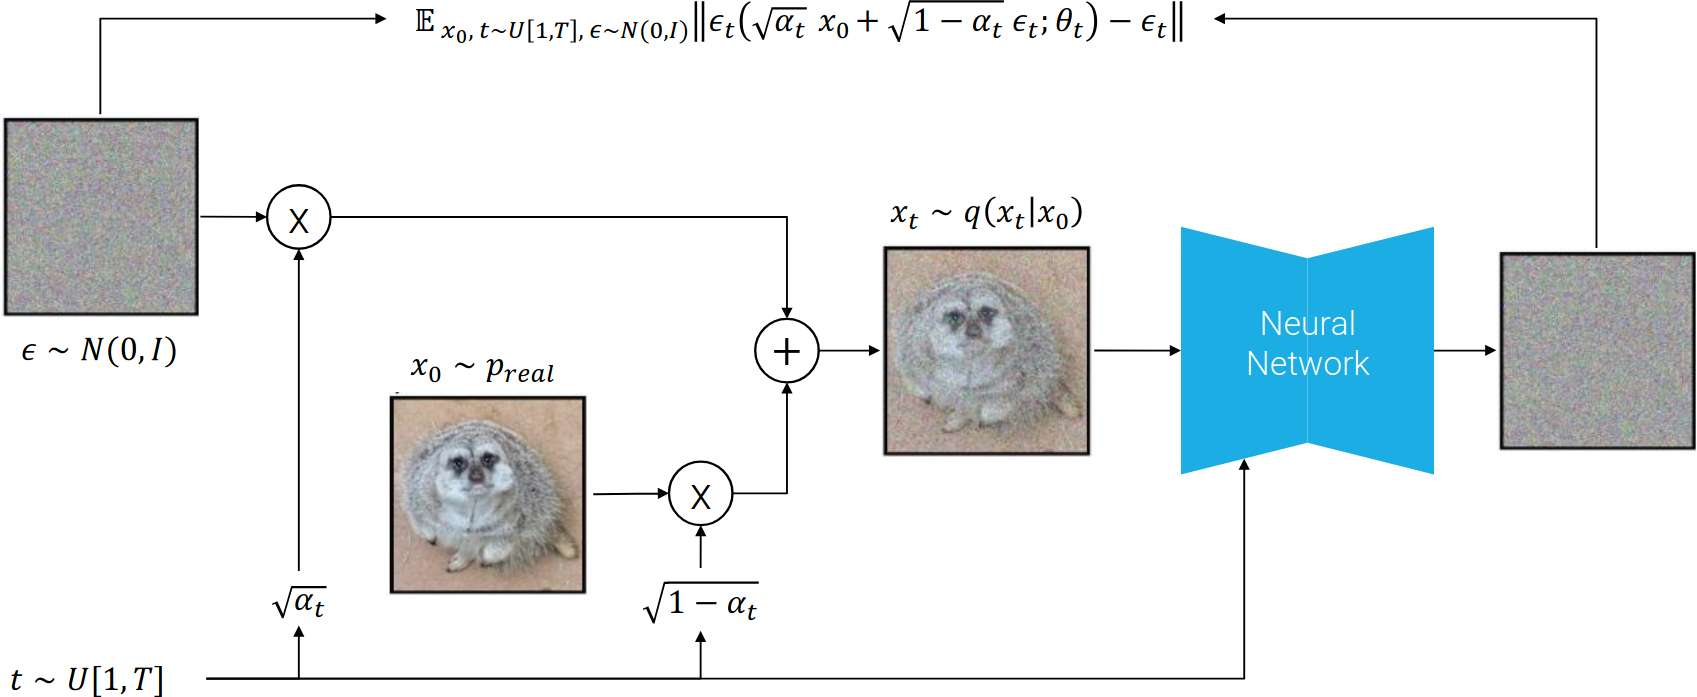
\includegraphics[width=0.9\linewidth]{./img/diffusion_model_training.jpg}
        \caption{Diffusion models training flow}
    \end{figure}
\end{description}


\subsection{Architecture}

\begin{description}
    \item[Generation architecture]
        Standard U-Net or transformer to predict the noise.

        \begin{description}
            \item[U-Net with self-attention]
                Add global self-attention at the layers of the backbone where the resolution of the image is sufficiently small. It is applied as follows:
                \begin{enumerate}
                    \item Flatten the spatial dimension to obtain $C$ 1D activations.
                    \item Pass the flattened activations through the self-attention layer.
                    \item Reshape the output to match the original activation.
                \end{enumerate}

                \begin{figure}[H]
                    \centering
                    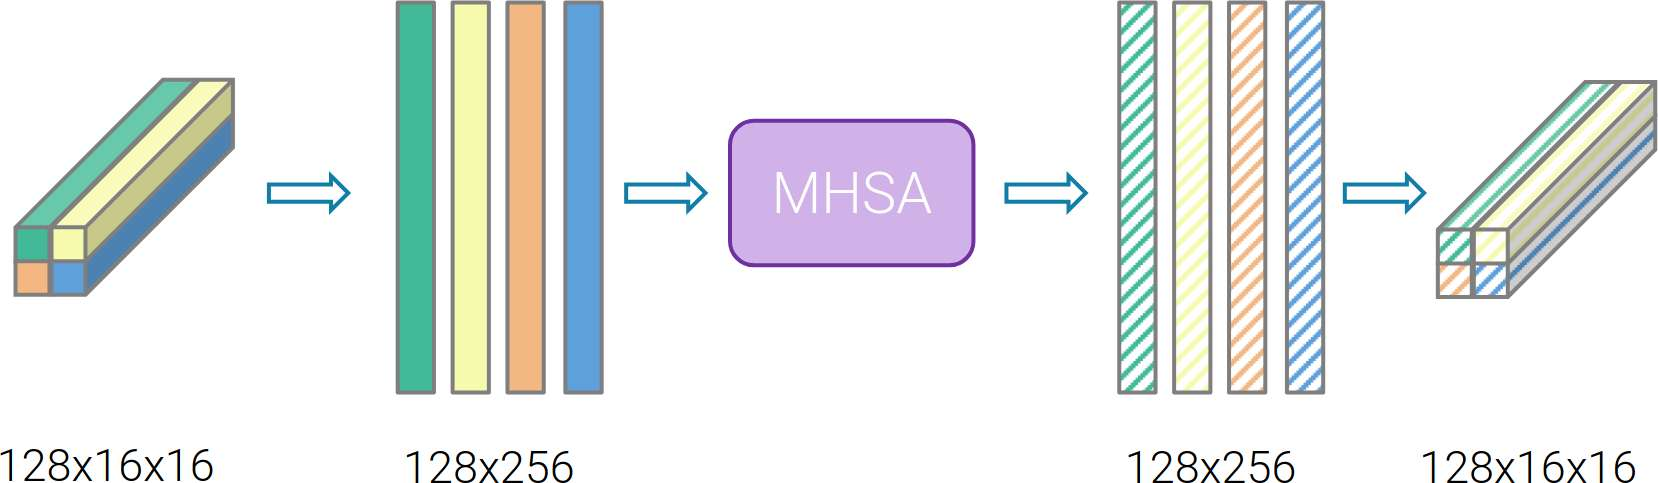
\includegraphics[width=0.7\linewidth]{./img/unet_attention.jpg}
                \end{figure}
        \end{description}
\end{description}


\begin{description}
    \item[Time conditioning] \marginnote{Time conditioning}
        In practice, the same network with the same set of weights is used to process each time step. Therefore, some time information has to be injected.

        Use transformer positional encoding, refined through some fully-connected layers to obtain an activation encoding time information. Then, two approaches are possible:
        \begin{descriptionlist}
            \item[Concatenation] 
                The time activation is concatenated along every spatial dimension of the image activations.

                \begin{figure}[H]
                    \centering
                    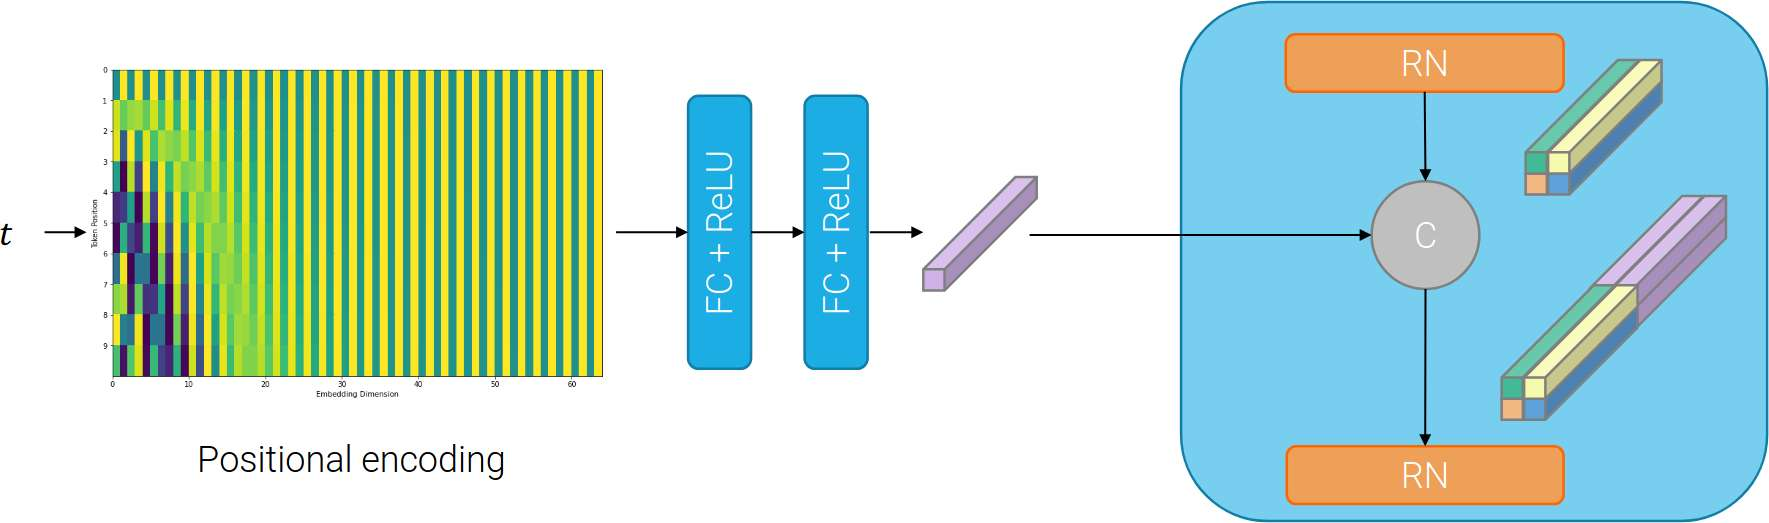
\includegraphics[width=0.75\linewidth]{./img/diffusion_model_time_conditioning1.jpg}
                \end{figure}

            \item[Adaptive group normalization] 
                The time activation is used as the modulator for adaptive group normalization (similar mechanism to AdaIN).

                \begin{figure}[H]
                    \centering
                    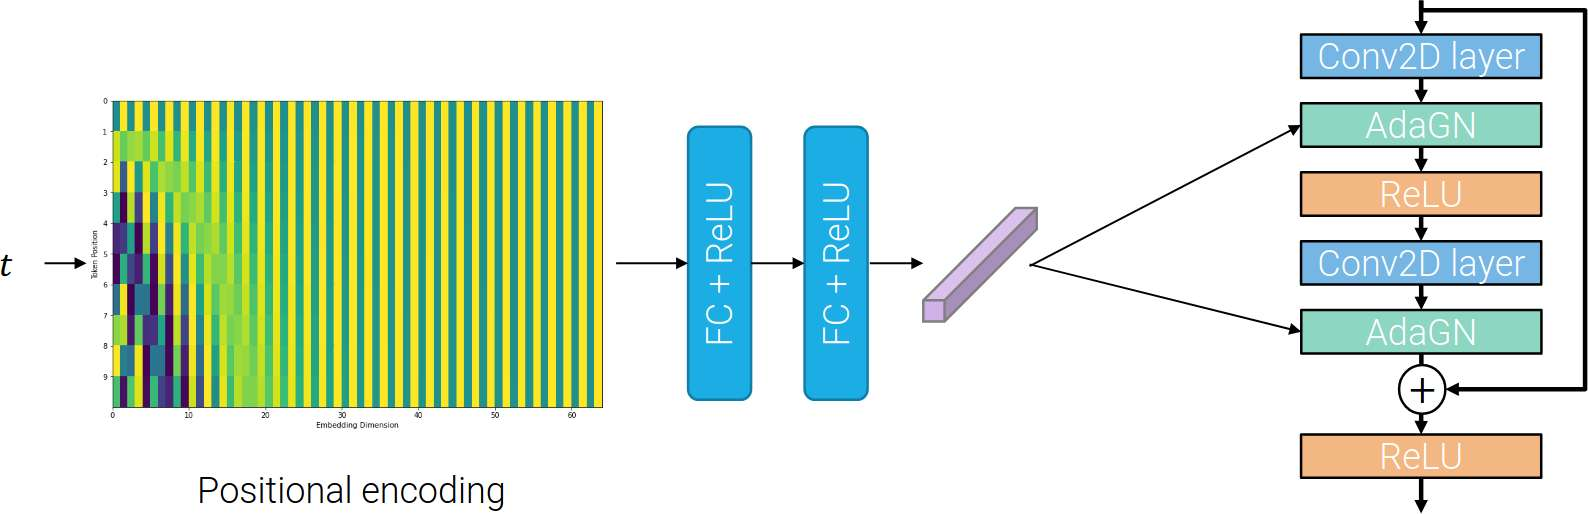
\includegraphics[width=0.75\linewidth]{./img/diffusion_model_time_conditioning2.jpg}
                \end{figure}
        \end{descriptionlist}
\end{description}


\subsection{Inference}

\begin{description}
    \item[Denoising diffusion probabilistic model (DDPM)] \marginnote{Denoising diffusion probabilistic model (DDPM)}
        Given a random latent $\x_T \sim \mathcal{N}(0; \matr{I})$, generation is done as follows:
        \begin{enumerate}
            \item For $t = T, \dots, 2$:
                \begin{enumerate}
                    \item Compute the mean of $p(\x_{t-1} \mid \x_t)$ by predicting the noise:
                    \[ \matr{\mu}_t = \frac{1}{\sqrt{1-\beta_t}}\x_t - \frac{\beta_t}{\sqrt{1-\alpha_{t-1}}\sqrt{1-\beta_t}} \varepsilon_t(\x_t; \matr{\theta}) \]
                    \item Sample the next less noisy image from $p(\x_{t-1} \mid \x_t)$:
                    \[ \x_{t-1} = \matr{\mu}_t + \sigma_t \noise_t \qquad \text{with } \noise_t \sim \mathcal{N}(0; \matr{I}) \]
                \end{enumerate}
            \item Use the mean of $p(\x_0 \mid \x_1)$ as the output image:
            \[ \x_0 = \frac{1}{\sqrt{1-\beta_t}}\x_1 - \frac{\beta_1}{\sqrt{1-\alpha_{0}}\sqrt{1-\beta_1}} \varepsilon_1(\x_1; \matr{\theta}) \]
        \end{enumerate}

        \begin{remark}
            In the original paper, a linear schedule for $\beta_t$ has been used. This results in a schedule for $\alpha_t$ that made the image mostly noise very quickly.

            \begin{figure}[H]
                \centering
                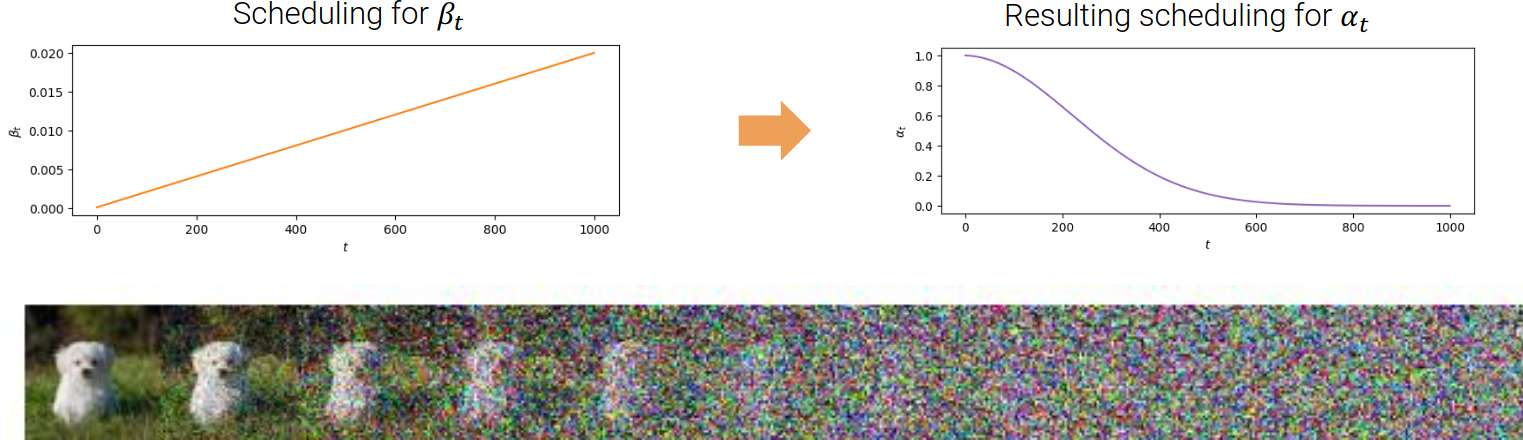
\includegraphics[width=0.9\linewidth]{./img/ddpm_schedule.jpg}
            \end{figure}
        \end{remark}

    \item[Improved DDPM (IDDPM)] \marginnote{Improved DDPM (IDDPM)}
        Use a cosine schedule for $\alpha_t$ (with $\beta_t = 1-\frac{\alpha_t}{\alpha_{t-1}}$) so that the trajectory does not destroy the image too quickly.
        \begin{figure}[H]
            \centering
            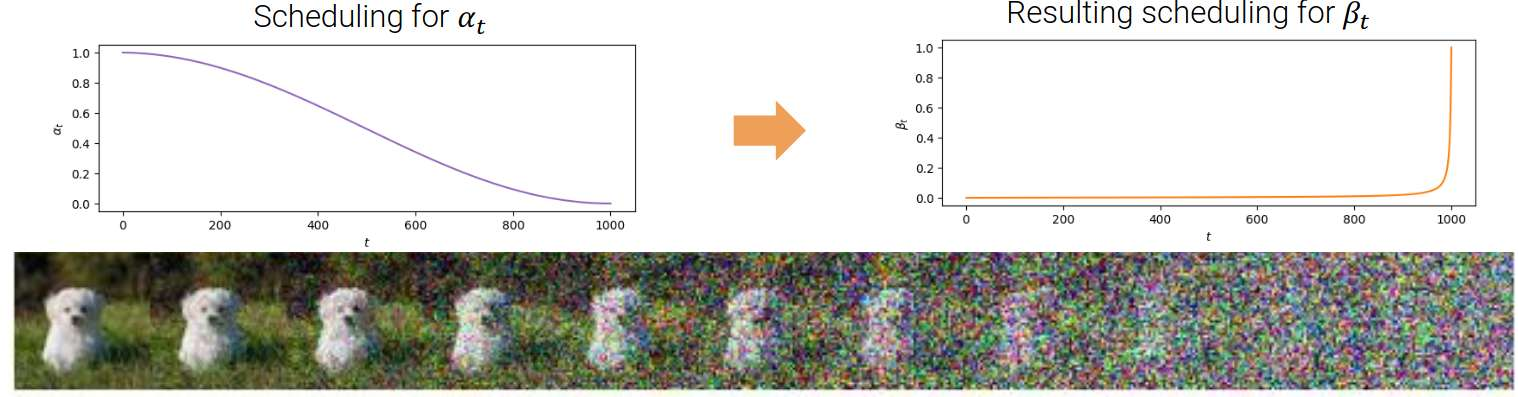
\includegraphics[width=0.85\linewidth]{./img/iddpm_schedule.jpg}
        \end{figure}
\end{description}

\begin{remark}
    The loss of diffusion models (with DDPM) only considers the marginal $q(\x_t \mid \x_0)$:
    \[ \sum_{i=1}^{I} \Bigg( \sum_{t=1}^{T} \frac{\beta_t^2}{(\alpha_{t-1})(1-\beta_t)} \Big\Vert \varepsilon_t
    \big( \underbrace{\sqrt{\alpha_t} \x_0^{(i)} + \sqrt{1-\alpha_t} \noise_t; \params_t}_\text{Sampled from $q(\x_t \mid \x_0)$} \big)
     - \noise_t \Big\Vert^2 \Bigg) \]
    Therefore, any new family of forward processes that use this same diffusion kernel (i.e., able to sample $\x_t$ conditioned to only $\x_0$) can reuse a pre-trained DDPM model.
\end{remark}

\begin{description}
    \item[Denoising diffusion implicit model (DDIM)] \marginnote{Denoising diffusion implicit model (DDIM)}
        \begin{description}
            \item[Forward process] 
                Use a family of non-Markovian forward distributions conditioned on the real image $\x_0$ and parametrized by a positive standard deviation $\vec{\sigma}$ defined as:
                \[ q_\vec{\sigma}(\x_1, \dots, \x_T \mid \x_0) = q_{\sigma_T}(\x_T \mid \x_0) \prod_{t=2}^{T} q_{\sigma_t}(\x_{t-1} \mid \x_t, \x_0) \]
                where:
                \[
                    \begin{gathered}
                        q_{\sigma_T}(\x_T \mid \x_0) = \mathcal{N}(0, \matr{I}) \\
                        q_{\sigma_t}(\x_{t-1} \mid \x_t, \x_0) = \mathcal{N}\left( \sqrt{\alpha_{t-1}}\x_0 + \sqrt{1-\alpha_{t-1}-\alpha_t^2} \frac{\x_t - \sqrt{\alpha_t} \x_0}{\sqrt{1-\alpha_t}}; \sigma_t^2\matr{I} \right)
                    \end{gathered}
                \]

                With this definition, it can be shown that:
                \[ q_{\sigma_t}(\x_t \mid \x_0) = \mathcal{N}(\sqrt{\alpha_t}\x_0; (1-\alpha_t)\matr{I}) \]

                \begin{remark}
                    With a specific choice for $\vec{\sigma}$ ($\sigma_t = \sqrt{\frac{1-\alpha_{t-1}}{1-\alpha_t}}\sqrt{1-\frac{\alpha_t}{\alpha_{t-1}}}$), it is possible to obtain DDPM (i.e., DDIM is a generalization of DDPM).

                    In practice, instead of tuning $\sigma_t$ directly, a proxy hyperparameter $\eta$ is used as follows:
                    \[ \sigma_t(\eta) = \eta \sqrt{\frac{1-\alpha_{t-1}}{1-\alpha_t}}\sqrt{1-\frac{\alpha_t}{\alpha_{t-1}}} \] 
                    In other words, $\eta$ controls $\sigma_t$ using the DDPM model as reference (with $\eta=1$ resulting in DDPM).
                \end{remark}

                \begin{remark}
                    With $\sigma_t \rightarrow 0$, the generation process becomes more deterministic. With $\sigma_t = 0$ ($\eta=0$), the mean is always sampled (i.e., fully deterministic).
                \end{remark}

                \begin{figure}[H]
                    \centering
                    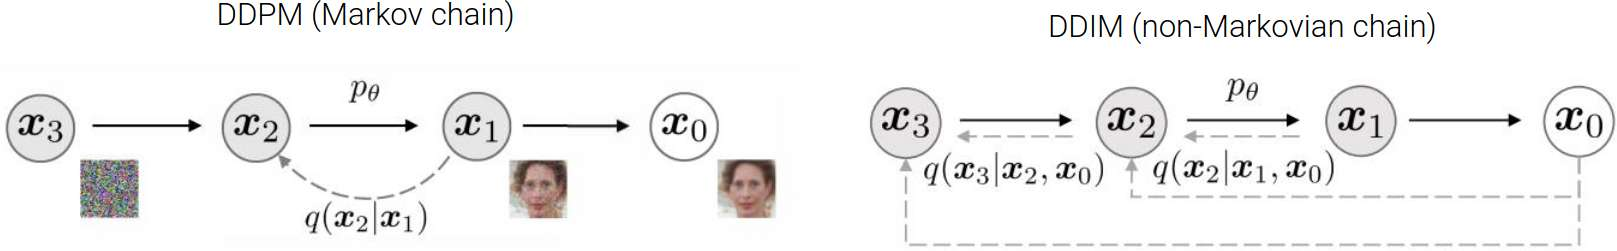
\includegraphics[width=0.9\linewidth]{./img/non_markovian_forward.jpg}
                \end{figure}

            \item[Reverse process] 
                Given a latent $\x_t$ and a DDPM model $\varepsilon_t(\cdot; \params)$, generation at time step $t$ is done as follows:
                \begin{enumerate}
                    \item Compute an estimate of the real image for the current time step $t$:
                    \[ \hat{\x}_0 = \frac{\x_t - \sqrt{\alpha_{t-1}} \varepsilon_t(\x_t; \params)}{\sqrt{\alpha_t}} = f_\params(\x_t) \]
                    Note that the formula comes from the usual $\x_t = \sqrt{\alpha_t}\x_0 + \sqrt{1-\alpha_t}\noise_t$.
                    \item Sample the next image from:
                    \[ p_\params(\x_{t-1} \mid \x_t) = q_\vec{\sigma}(\x_{t-1} \mid \x_t, f_\params(\x_t)) \]
                    (i.e., $\x_0$ in $q_\vec{\sigma}$ has been replaced with an estimation of it).
                    The image is obtained as:
                    \[ \x_{t-1} = \matr{\mu}_{q_\vec{\sigma}} + \matr{\Sigma}_{q_\vec{\sigma}} \noise \]
                \end{enumerate}

            \item[Accelerate sampling] \marginnote{Accelerate sampling}
                Use a forward process that only considers a subset of time steps. This allows to skip $k$ steps in the reverse process as:
                \[ 
                    \begin{split}
                        p_\params(\x_{t-k} \mid \x_t) &= q_\vec{\sigma}(\x_{t-k} \mid \x_t, \x_0) \\
                        &= \mathcal{N}\left( \sqrt{\alpha_{t-k}}\x_0 + \sqrt{1-\alpha_{t-k}-\sigma_t^2} \frac{\x_t-\sqrt{\alpha_t}\x_0}{\sqrt{1-\alpha_t}}; \sigma_t^2\matr{I} \right) 
                    \end{split}
                \] 

                \begin{remark}
                    Skipped steps are actually present in the forward process as during training all steps are considered. Therefore, it is only possible to skip steps during inference.
                \end{remark}

                \begin{remark}
                    It has been observed that determinism ($\sigma_t=0$/$\eta=0$) with accelerated generation has the best performance.
                \end{remark}

                \begin{figure}[H]
                    \centering
                    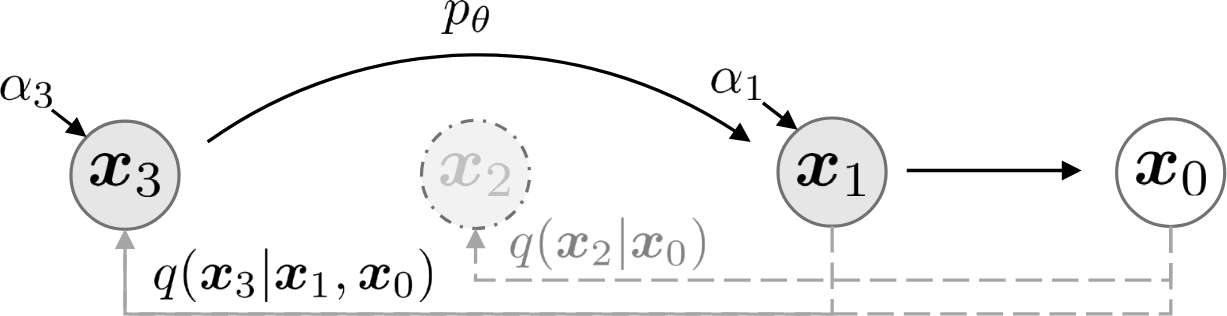
\includegraphics[width=0.45\linewidth]{./img/diffusion_accelerated_sampling.jpg}
                \end{figure}
        \end{description}
\end{description}


\subsection{Interpretation of diffusion models as score estimators}

\begin{description}
    \item[Score function] \marginnote{Score function}
        Given a probability density function $p(x)$, its score function is defined as:
        \[ s(x) = \nabla_x\left[ \log(p(x)) \right] \]

        \begin{remark}
            Differently from a probability distribution, the score function $s$ does not have to be normalized to sum $1$. Therefore, it is easier to approximate with a neural network $s(x; \theta)$.
        \end{remark}

        \begin{figure}[H]
            \centering
            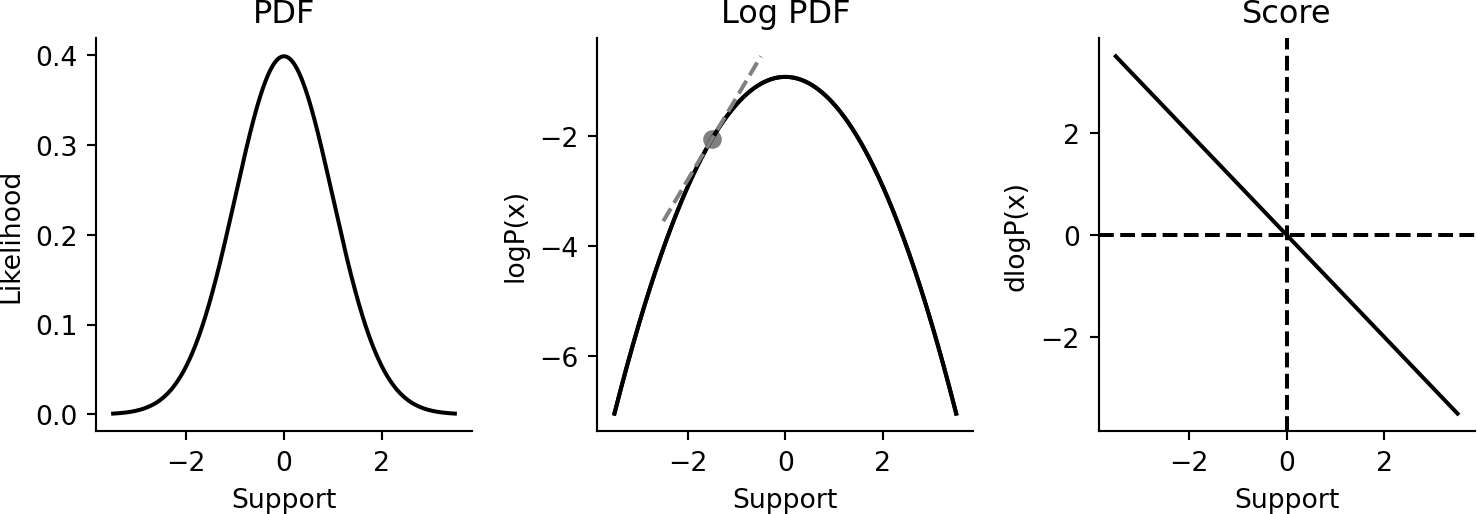
\includegraphics[width=0.65\linewidth]{./img/score_function.jpg}
        \end{figure}

        The score function indicates which direction maximally increases $p(x)$. In other words, it defines a vector field that points towards the modes of $p(x)$.

    \item[Langevin dynamics] \marginnote{Langevin dynamics}
        Method to sample from a score function as:
        \[ \x_{t-1} = \x_t + c \nabla_\x\left[ \log(p(x)) \right] + \sqrt{2c} \noise \]
        where $c$ is a hyperparameter.

        \begin{figure}[H]
            \centering
            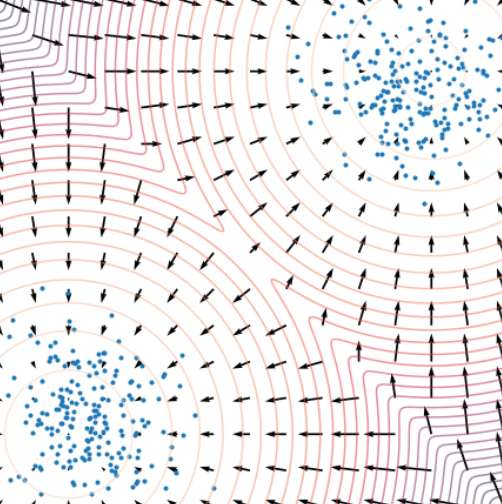
\includegraphics[width=0.3\linewidth]{./img/langevin_dynamics.jpg}
        \end{figure}

        \begin{remark}
            Score functions are inaccurate in low density regions. Therefore, sampling is inaccurate in areas with fewer data points.

            \begin{figure}[H]
                \centering
                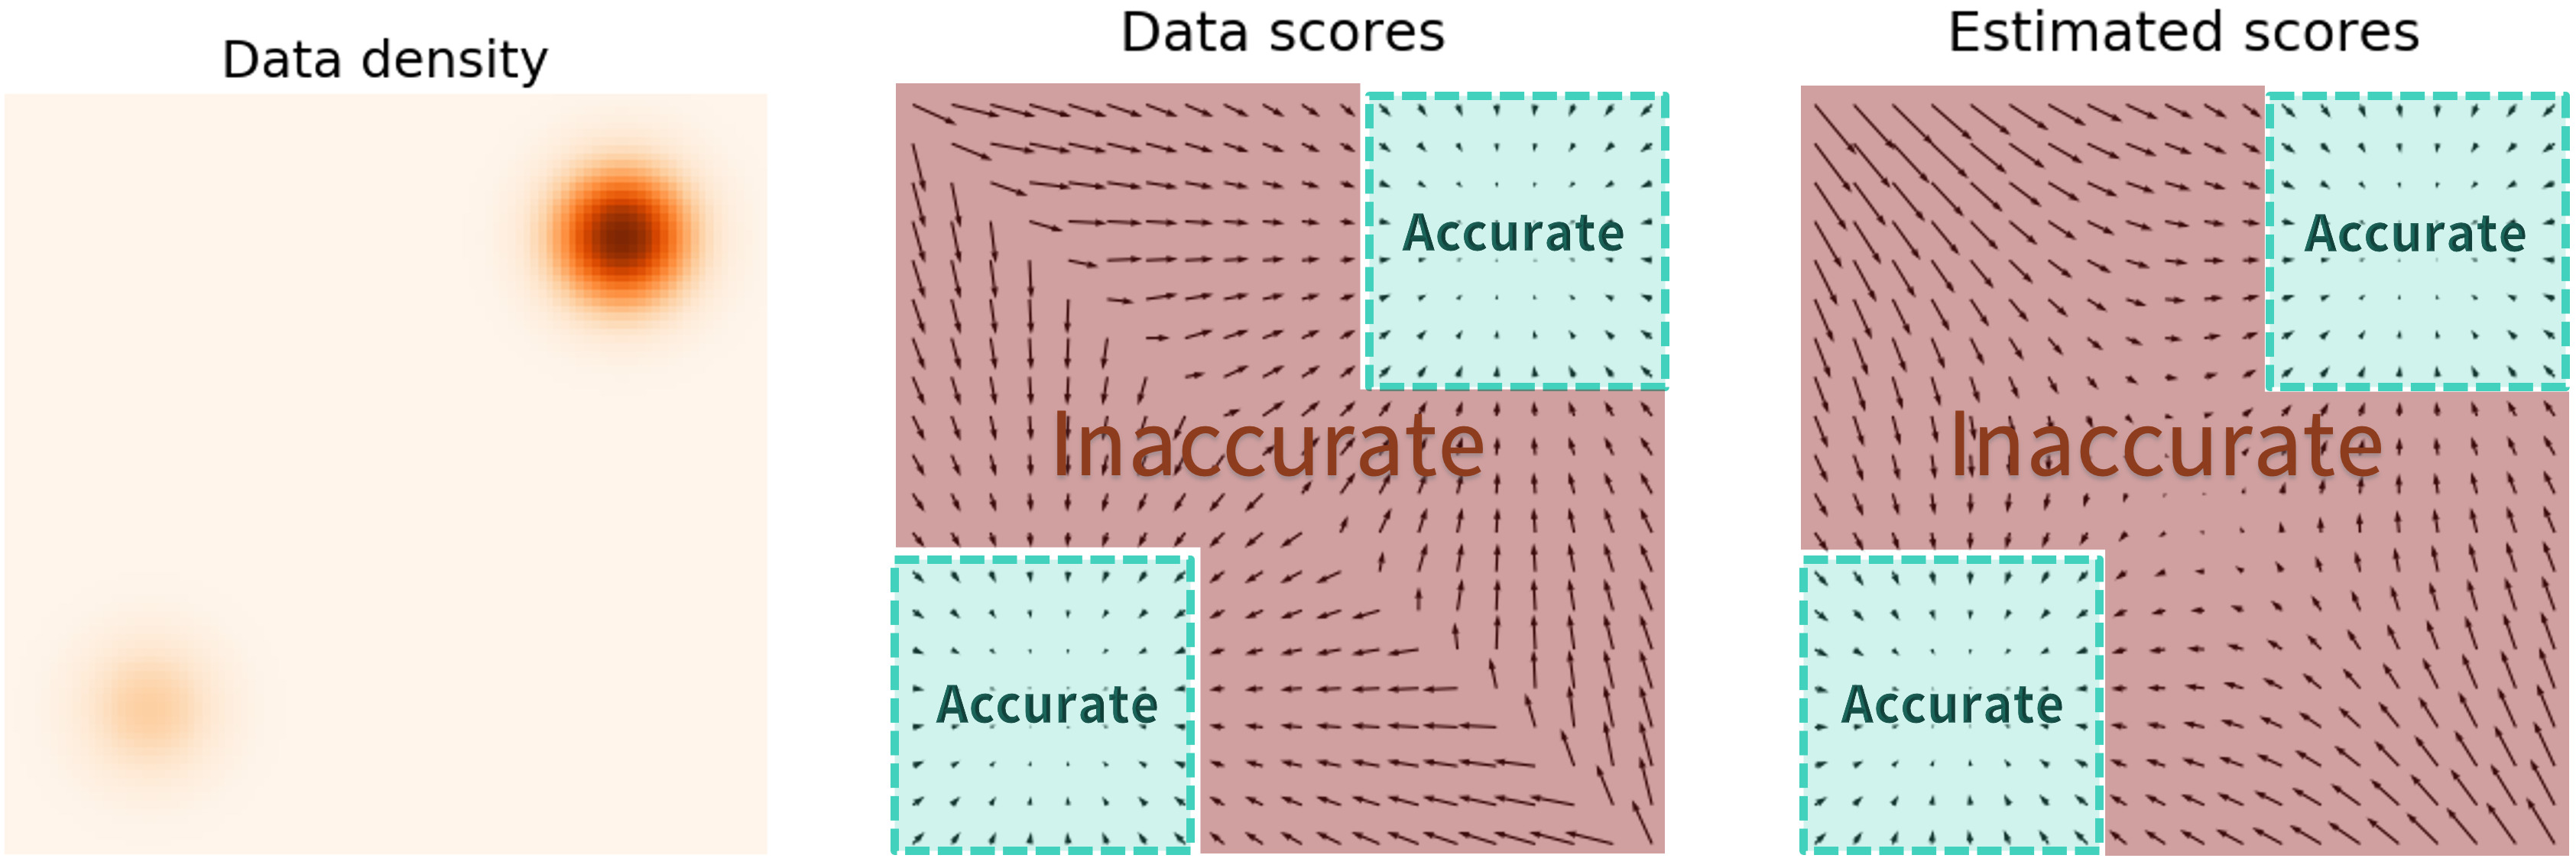
\includegraphics[width=0.65\linewidth]{./img/langevin_dynamics_low_density.jpg}
            \end{figure}
        \end{remark}

    \item[Langevin dynamics with noise] \marginnote{Langevin dynamics with noise}
        Add noise to the original data to make the trained score function more robust.

        \begin{figure}[H]
            \centering
            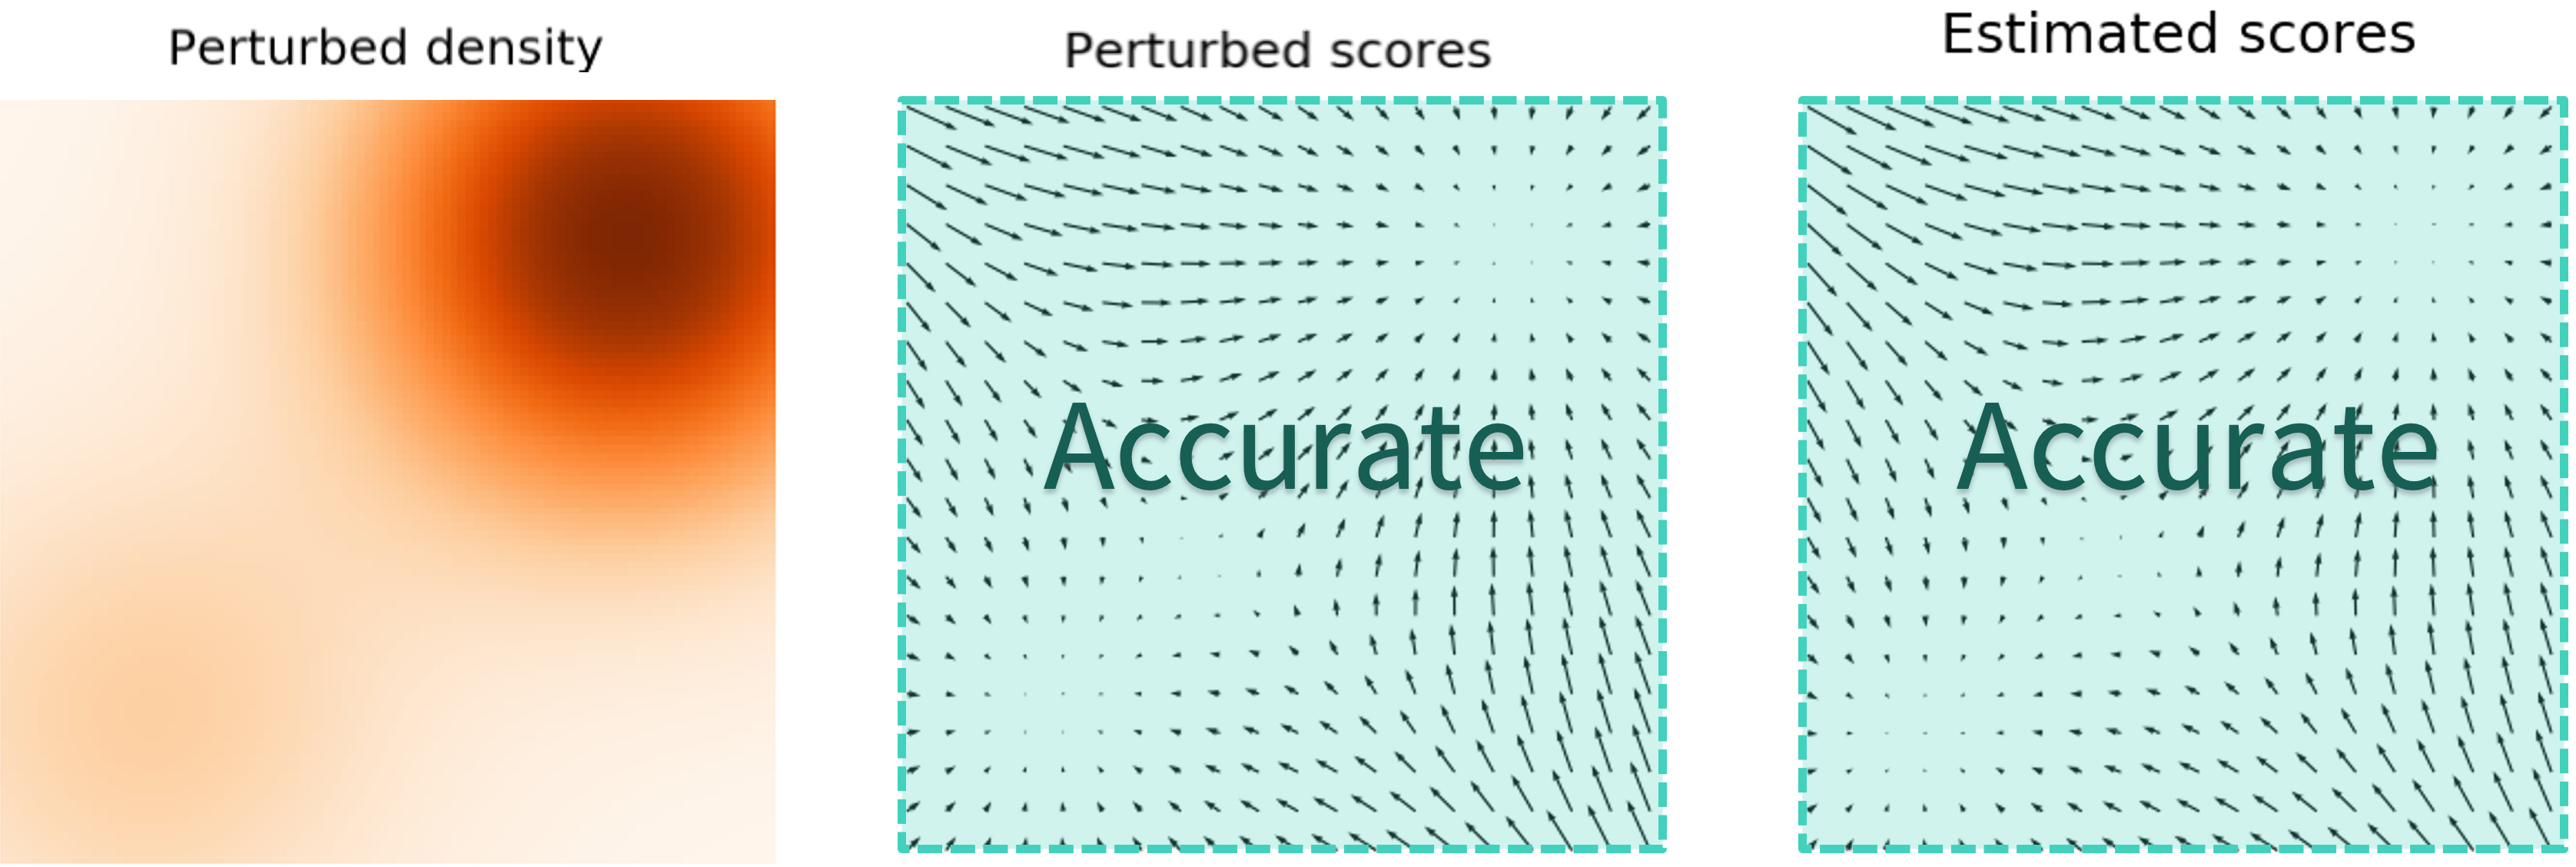
\includegraphics[width=0.6\linewidth]{./img/langevin_dynamics_noise.jpg}
        \end{figure}

        \begin{remark}
            Larger scales of noise significantly alter the original distribution. Smaller scales of noise do not cover enough low density regions.
        \end{remark}

        \begin{description}
            \item[Annealed Langevin dynamics] \marginnote{Annealed Langevin dynamics}
                Use multiple scales of noise to estimate a family of score functions $s_t(\x_t; \params)$. Then, run a few steps of Langevin dynamics for $t=T, \dots, 1$, each time restarting from $t-1$.

                \begin{figure}[H]
                    \centering
                    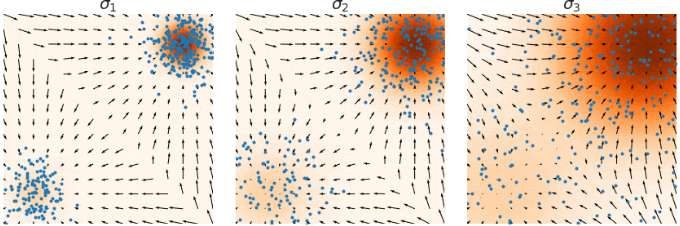
\includegraphics[width=0.7\linewidth]{./img/annealed_langevin_dynamics.jpg}
                \end{figure}
        \end{description}

    \item[Diffusion model as score estimator]
        The score function of an isotropic Gaussian distribution is:
        \[ 
            \begin{split}
                s(\x) &= \nabla_\x\left[ \log(p(\x)) \right] \qquad \text{with } \x \sim p(\x) = \mathcal{N}(\matr{\mu}; \sigma^2\matr{I}) \\
                &= \nabla_\x\left[ \log\left( \frac{1}{c} e^{-\frac{(\x-\matr{\mu})^2}{2\sigma^2}} \right) \right] \\
                &= \nabla_\x\left[ \log\left(\frac{1}{c}\right) \right] + \nabla_\x\left[ -\frac{(\x - \matr{\mu})^2}{2\sigma^2} \right] \\
                &= -\frac{\x - \matr{\mu}}{\sigma^2}
            \end{split}
        \]
        As it holds that:
        \[ \x = \matr{\mu} + \sigma\noise \iff \noise = \frac{\x - \matr{\mu}}{\sigma} \qquad \text{with } \noise \sim \mathcal{N}(0; \matr{I}) \]
        The score function can be rewritten as an estimator of the Gaussian noise:
        \[ s(\x) = -\frac{\x - \matr{\mu}}{\sigma^2} = -\frac{\noise}{\sigma} \]
        Therefore, as diffusion models learn to predict $\varepsilon_t(\x_t; \params)$ from a Gaussian with $\sigma = \sqrt{1-\alpha_t}$, they can be seen as score functions with a scaling factor $-\sigma$:
        \[ 
            s(\x) = -\frac{\varepsilon_t(\x_t; \params)}{\sqrt{1-\alpha_t}} \iff 
            \varepsilon_t(\x_t; \params) = -\sqrt{1-\alpha_t} s(\x)
        \]

        As a result, diffusion models implicitly perform annealed Langevin dynamics when generating an image.

        \begin{figure}[H]
            \centering
            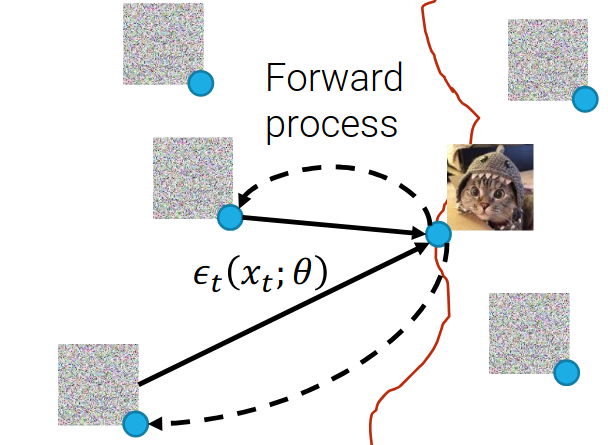
\includegraphics[width=0.3\linewidth]{./img/diffusion_model_annealing.png}
        \end{figure}
\end{description}


\subsection{Generation conditioning}

\begin{description}
    \item[One-hot class conditioning] \marginnote{One-hot class conditioning}
        Condition generation based on a class $c$. The model predicting noise becomes:
        \[ \varepsilon_t(\x_t, c; \params) \]
        Architecturally, similarly to time conditioning, the one-hot encoding of the class is refined through fully-connected layers to create an embedding that is appended to the image activations.

        \begin{remark}
            This works as conditioning the likelihood with a class $c$ does not change the previous proofs.
        \end{remark}

        \begin{description}
            \item[Cascaded diffusion models] \marginnote{Cascaded diffusion models}
                Approach to generate high resolution images starting from some class conditioning.

                Given a standard diffusion model $d_1$ and a series of super-resolution diffusion models $d_2, \dots, d_n$ with increasing resolution, the generation of an image of class $c$ is done as follows:
                \begin{enumerate}
                    \item Use the first diffusion model $d_1$ to generate a starting low-resolution image $\matr{I}_1$ from a latent and the class $c$.
                    \item Iterate over the super-resolution diffusion models $i=2, \dots, n$:
                    \begin{enumerate}
                        \item Up-sample the previously generated image $\matr{I}_{i-1}$ to match the shape of the current diffusion model $d_i$.
                        \item Generate a higher resolution image $\matr{I}_i$ using the diffusion model $d_i$ from a latent conditioned on the class $c$ and the previous image $\matr{I}_{i-1}$ (which is concatenated along the spatial dimension of the latent).
                    \end{enumerate}
                \end{enumerate}

            \begin{remark}
                Higher-resolution models in the pipeline can be seen as detail generators.
            \end{remark}

            \begin{figure}[H]
                \centering
                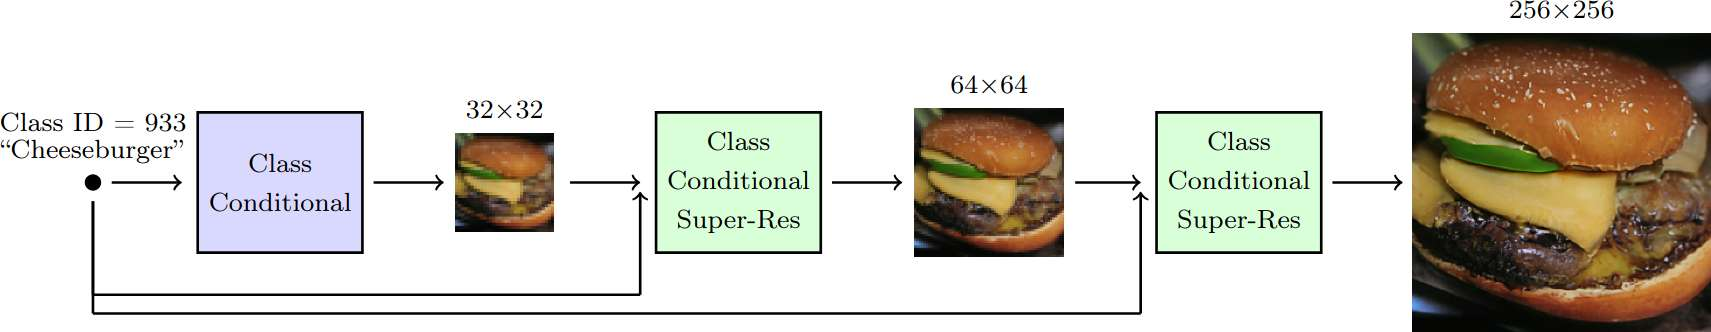
\includegraphics[width=0.9\linewidth]{./img/cascaded_diffusion_models.jpg}
            \end{figure}
        \end{description}

    \item[Classifier guidance] \marginnote{Classifier guidance}
        Use a classifier to compute $p_\text{cls}(c \mid \x_t, t)$ and guide generation to a class $c$. With the interpretation of diffusion models as score estimators, the classifier is used to steer the trajectories of Langevin dynamics given the latent $\x_t$ at time $t$.

        Given a latent classifier, the class-guided noise can be predicted as follows:
        \[
            \begin{split}
                \varepsilon_t^{\text{cls}}(\x_t, c; \params) 
                &= -\sqrt{1-\alpha_t} \nabla_{x_t}\Big[ \log(p(\x_t, c)) \Big] \\
                &= -\sqrt{1-\alpha_t} \nabla_{x_t}\Big[ \log\big(p(\x_t) p_\text{cls}(c \mid \x_t, t)\big) \Big] \\
                &= -\sqrt{1-\alpha_t} \nabla_{x_t}[ \log(p(\x_t)) ] - \sqrt{1-\alpha_t} \nabla_{x_t}[ \log(p_\text{cls}(c \mid \x_t, t)) ] \\
                &= -\sqrt{1-\alpha_t} s(\x_t) - \sqrt{1-\alpha_t} \nabla_{x_t}[ \log(p_\text{cls}(c \mid \x_t, t)) ] \\
                &= \varepsilon_t(\x_t; \params) - \sqrt{1-\alpha_t} \nabla_{x_t}[ \log(p_\text{cls}(c \mid \x_t, t)) ]
            \end{split}
        \]
        In practice, a weight $w$ is used to control the strength of guidance:
        \[ \varepsilon_t^{\text{cls}}(\x_t, c; \params) = \varepsilon_t(\x_t; \params) - w \nabla_{x_t}[ \log(p_\text{cls}(c \mid \x_t, t)) ] \]

        \begin{remark}
            Guidance allows to balance the trade-off between realism and coverage (in a better way than one-hot conditioning).
        \end{remark}

        \begin{remark}
            The best results have been obtained by using an already conditional diffusion model. Therefore, $\varepsilon_t(\x_t, c; \params)$ can be substituted in place of $\varepsilon_t(\x_t; \params)$.
        \end{remark}

        \begin{remark}
            The classifier usually has to be trained on latents from scratch and it is domain specific.
        \end{remark}

    \item[Classifier-free guidance] \marginnote{Classifier-free guidance}
        Generation guidance method that does not require a classifier for latents.

        Consider the formulation of classifier guidance starting with a conditional generator: 
        \[
            \begin{split}
                \varepsilon_t^{\text{cls}}(\x_t, c; \params) 
                &= \varepsilon_t(\x_t, c; \params) - w \nabla_{x_t}[ \log(p_\text{cls}(c \mid \x_t, t)) ] \\
                % &= - \big( - \varepsilon_t(\x_t, c; \params) + w \nabla_{x_t}[ \log(p_\text{cls}(c \mid \x_t, t)) ] \big)
            \end{split}
        \]
        By applying Bayes' rule on the second term, we have that:
        \[
            \begin{split}
                w \nabla_{x_t}[ \log(p_\text{cls}(c \mid \x_t, t)) ]
                &= w \nabla_{x_t}\left[ \log\left( p(\x_t \mid c) \frac{p(c)}{p(\x_t)} \right) \right] \\
                &= w \nabla_{x_t}\left[ \log(p(\x_t \mid c)) \right] + w \nabla_{x_t}\left[ \log(p(c)) \right] - w \nabla_{x_t}\left[ \log(p(\x_t)) \right] \\
                &= w \nabla_{x_t}\left[ \log(p(\x_t \mid c)) \right] + 0 - w \nabla_{x_t}\left[ \log(p(\x_t)) \right] \\
                &\approx - w \varepsilon_t(\x_t, c; \params) + w \varepsilon_t(\x_t; \params)
            \end{split}
        \]
        Therefore, for guidance without a classifier, two models are required:
        \begin{itemize}
            \item A conditional generative model (i.e., $\varepsilon_t(\x_t, c; \params)$).
            \item An unconditional generative model (i.e., $\varepsilon_t(\x_t; \params)$).
        \end{itemize}
        The overall class guided noise is computed as:
        \[ 
            \begin{split}
                \varepsilon_t^{\text{cls}}(\x_t, c; \params) 
                &= \varepsilon_t(\x_t, c; \params) + w \varepsilon_t(\x_t, c; \params) - w \varepsilon_t(\x_t; \params) \\
                &= (1 + w) \varepsilon_t(\x_t, c; \params) - w \varepsilon_t(\x_t; \params)
            \end{split}
        \]

        \begin{remark}
            In practice, a single model is used for both conditional and unconditional generation.
        \end{remark}

        \begin{description}
            \item[Training]
                The model is trained as a one-hot class conditioned model. In addition, with probability $p_\text{uncond}$ (e.g., $0.1$), training is done unconditioned (i.e., the one-hot vector is zeroed).
        \end{description}

        \begin{remark}
            During inference, the model has to be run twice on the latent to compute the conditioned and unconditioned noise.
        \end{remark}

    \item[Text conditioning] \marginnote{Text conditioning}
        Embed text using an encoder and use the outputs at each token as keys and values of the cross-attentions in U-Net while the queries come from the image.

        \begin{description}
            \item[Training] 
                Similarly to classifier-free guidance, the model is trained both with and without a conditioning prompt.

                \begin{remark}
                    The training procedure can also be generalized to negative prompts.
                \end{remark}
        \end{description}

        \begin{figure}[H]
            \centering
            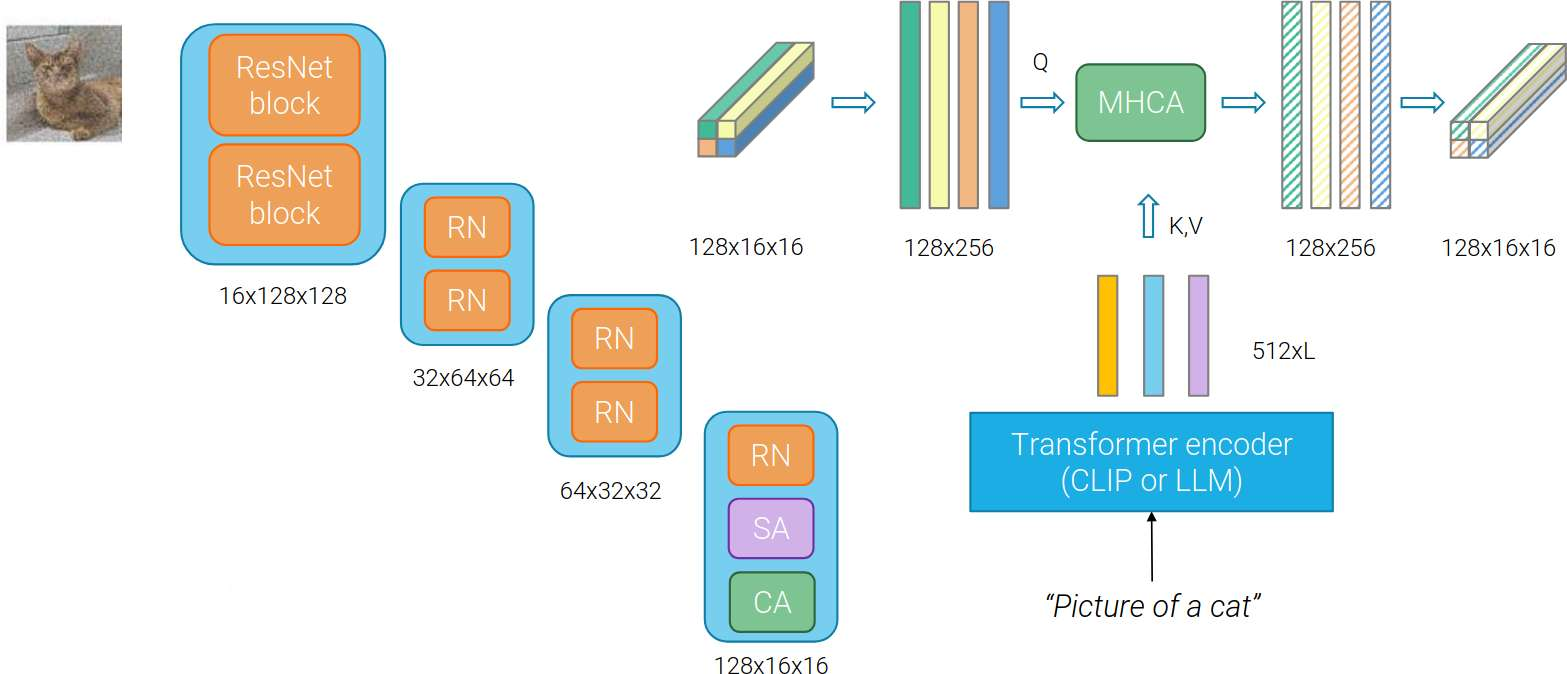
\includegraphics[width=0.75\linewidth]{./img/diffusion_text_conditioning.jpg}
        \end{figure}

        \begin{description}
            \item[Imagen] \marginnote{Imagen}
                Architecture based on the following steps:
                \begin{enumerate}
                    \item Embed a prompt using a frozen text encoder.
                    \item Generate an initial low-resolution image using a diffusion model that takes as input only the prompt.
                    \item Pass the low-resolution image and the prompt embeddings through a series of super-resolution diffusion models.
                \end{enumerate}

                \begin{figure}[H]
                    \centering
                    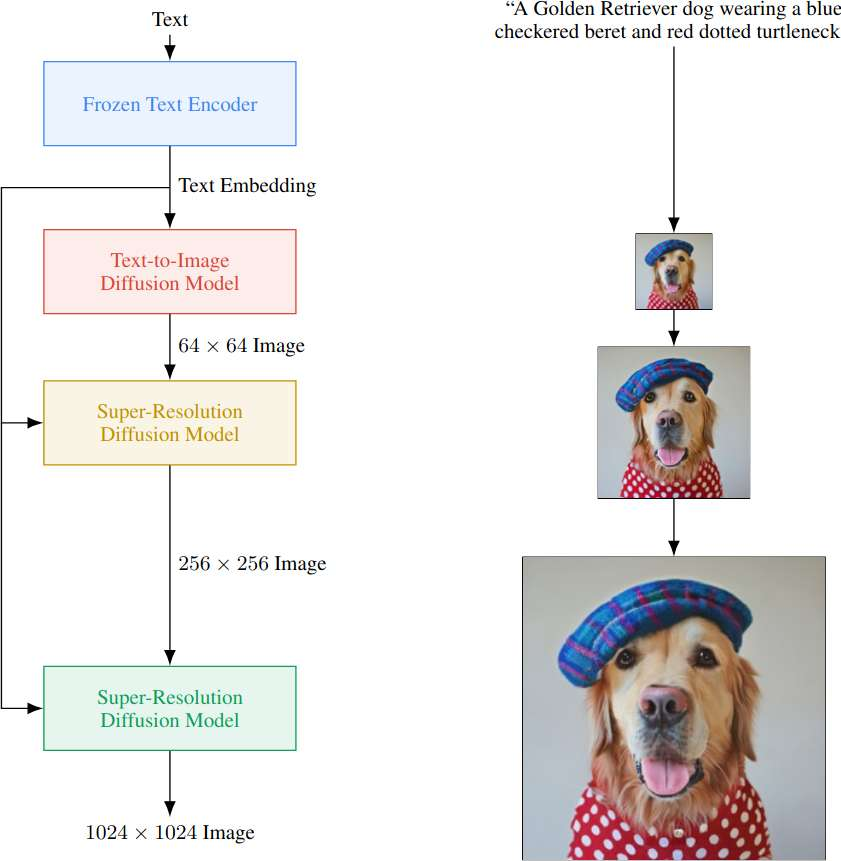
\includegraphics[width=0.4\linewidth]{./img/imagen.jpg}
                \end{figure}
        \end{description}
\end{description}


\subsection{Latent diffusion models}

\begin{description}
    \item[Latent diffusion model] \marginnote{Latent diffusion model}
        Use an autoencoder to generate a compressed latent image to pass through the diffusion model and decode it at the end of generation.

        \begin{figure}[H]
            \centering
            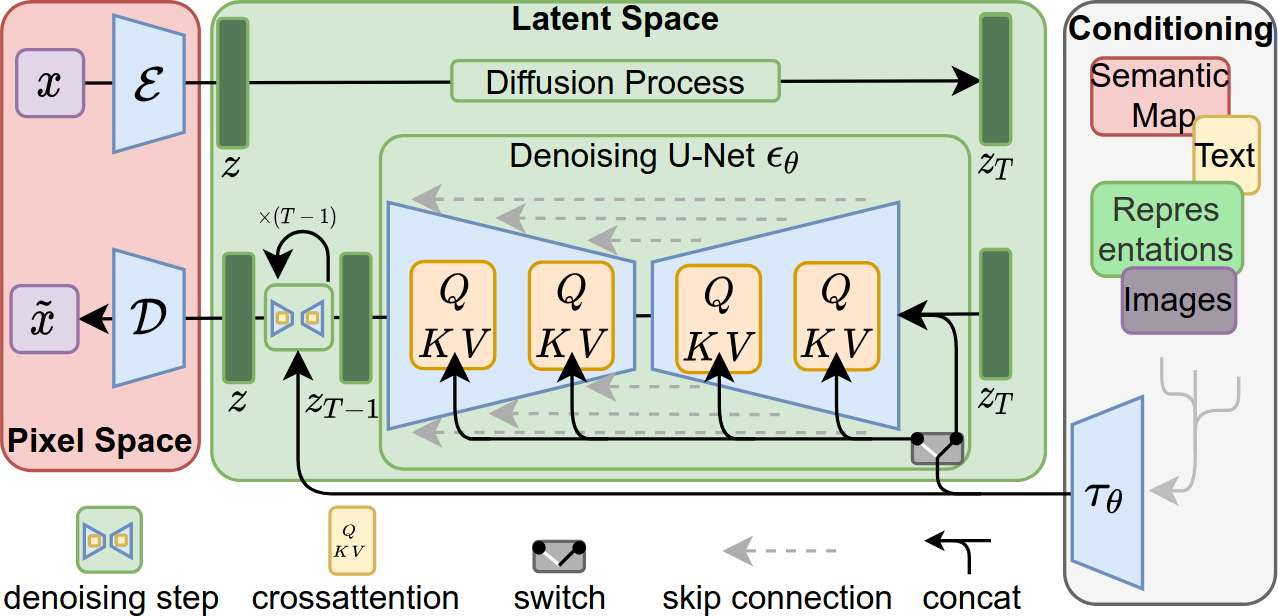
\includegraphics[width=0.55\linewidth]{./img/latent_diffusion.jpg}
        \end{figure}

        \begin{description}
            \item[Stable diffusion] \marginnote{Stable diffusion}
                Model based on latent diffusion with text conditioning.
        \end{description}
\end{description}


\let\x\undefined
\let\params\undefined